% ==================================================
\chapter{Methods}\label{chap:Methods }
% ==================================================

In this methods chapter, I will explain various criteria for evaluating academic performance, individual visualization (Scholar Plot), group visualization (Department Plot), and Academic Garden which is a scalable visualization of academic merit.


% --------------------------
\section{Design Process}
% --------------------------
There are various criteria for evaluating academic performance. I focus on three main criteria.
\begin{itemize}
\item \textbf{Impact} - it is the post-production merit. For example, the citations, in which a publication receives. A publication with a higher number of citations has higher visibility. Therefore, I linked the impact to the vertical axis in the plot.
\item \textbf{Prestige} - this is the pre-production merit associated with the venue of publication. For example, the impact factor of a journal is the merit your publication will acquire because it has been published in that journal. Hence, I associate a disk with variable sizes to the prestige of the venue. I consider it as a `fancy factor'.
\item \textbf{Funding} - it enables the production of publications/research. Hence, I placed it at the bottom of the plot. This can help to correlate the production with the funding.
\end{itemize}

ScholarPlot uses publicly available publication and affiliation information on researchers, scholars, and authors for the purpose of visualizing popular indicators of publishing activity. No single set of indicators can capture all of the dimensions of a publication's scholarly value or an author's contributions to knowledge. Depending on a user's objective, ScholarPlot may be best used in combination with other measures. The visualization consists of a hierarchy of visualization schemes right from the individual to the department and the college.









% =============================================================================
\section{Scholar Plot - Individual Visualization}
% =============================================================================
Scholar Plot obtains the Impact Factor ($IF$) \cite{garfield2006history} for a particular journal from our database. The data of Impact Factor is acquired from The Thomson Reuters Impact Factor - Web of Science \cite{Thoms79:online}. Based on all this information, it constructs the plots as per the design outlined in the Visualization and User Interface section, using nvd3 reusable charting library \cite{nvd3org} and d3.js JavaScript library \cite{d3js}.


The NSF/NIH/NASA funding datasets are available at the respective US government websites in various file formats such as XML, CSV, and so on \cite{nsf, nih}. I implemented a script \ref{code-xml} to parse this massive XML dataset into our data structure that consists of AwardID, AwardAmount, First name, Last name, Investigator by RoleCode (Principal Investigator, Co-Principal Investigator and Former Principal Investigator), using XMLStarlet \cite{XMLStarlet}. I imported this data to our database using Toad DBMS tool \cite{Toadf85:online}. %We designed our relational database schema in MySQL.

\begin{figure*}
    \centering
    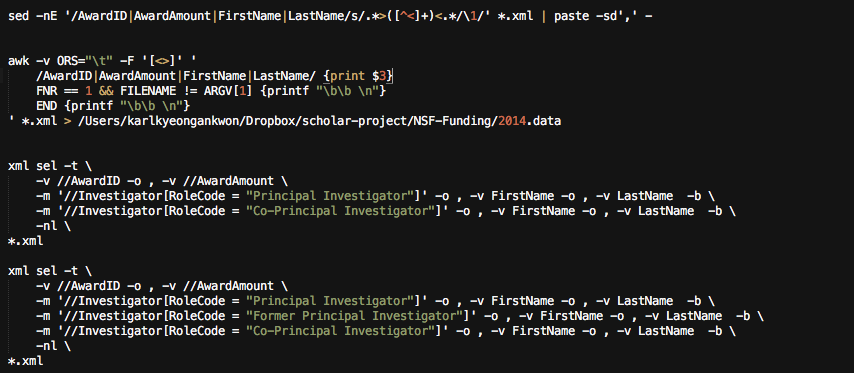
\includegraphics[width=1\textwidth]{figures/fig-code-xml.png}
    \caption{A code snippet of XMLStarlet.}~\label{code-xml}
\end{figure*}


\begin{figure}%[!htb]
\centering
  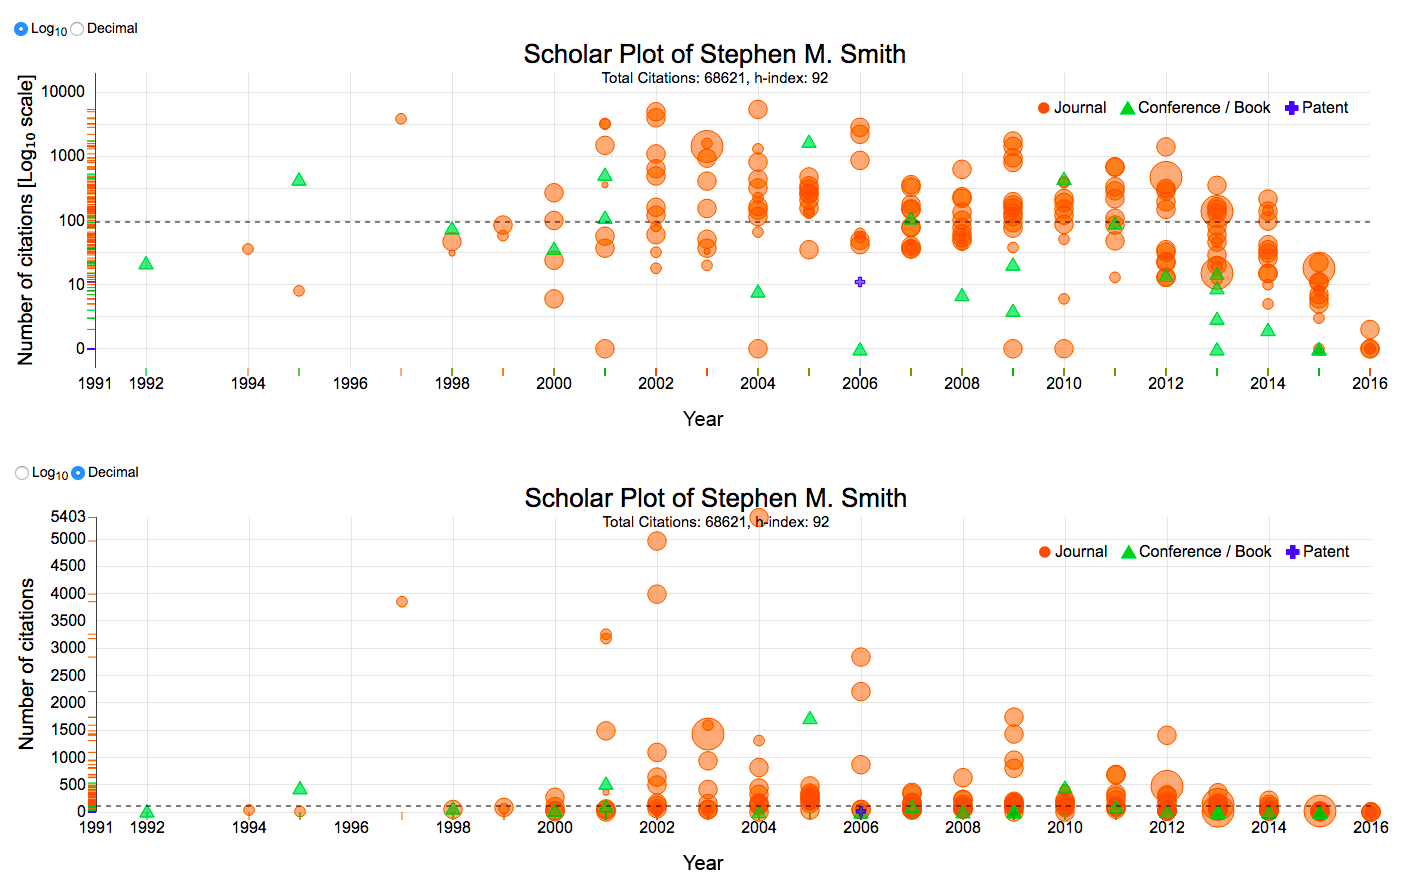
\includegraphics[width=1\textwidth]{figures/fig_scaleView-HD}
  \caption{An example of a senior records of the $log_{10}$ view and $decimal$ view - the radio button allows users to switch between different scale views without reloading the entire page. The two different scales view to create a standardized scale for the y-axis for comparison, $log_{10}$ scale is the default plot and an option to toggle to the decimal scale view.}~\label{fig-scale}
\end{figure}


\begin{figure*}
  \centering
  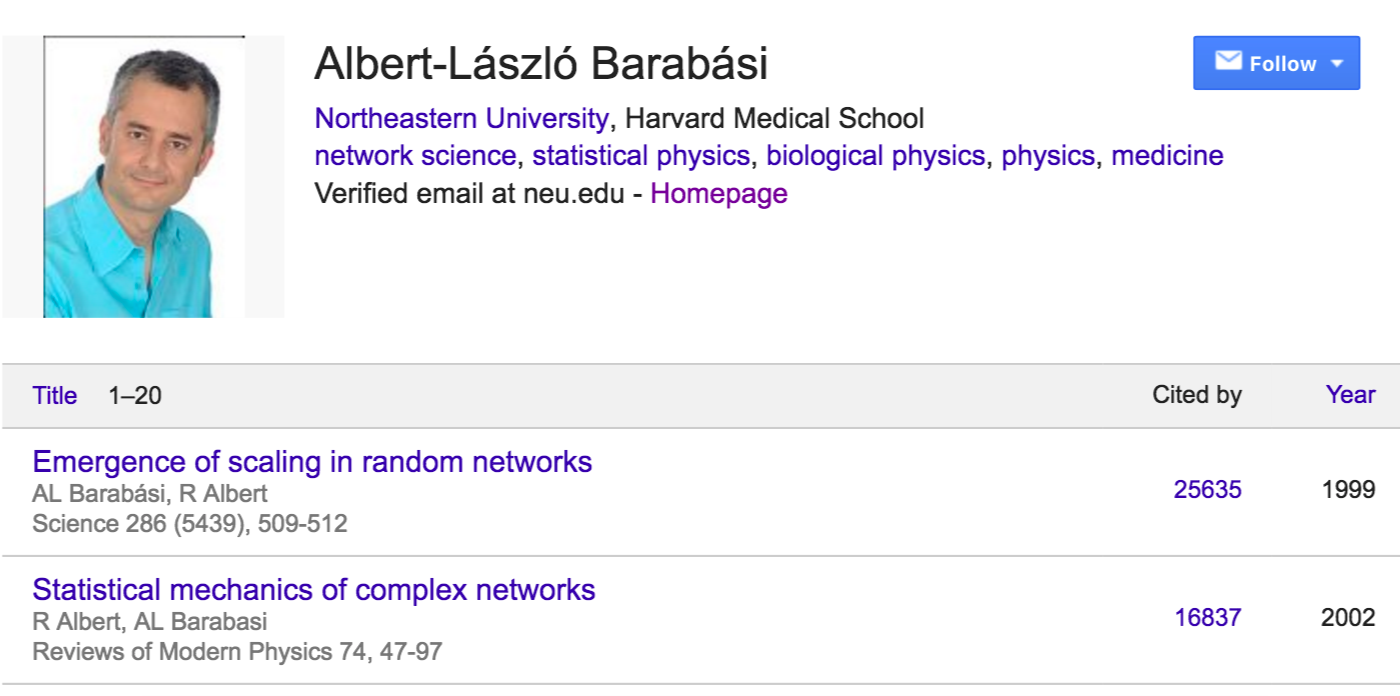
\includegraphics[width=.8\textwidth]{figures/fig_publication-1}
  
\includegraphics[width=.8\textwidth]{figures/fig_publication-2}
  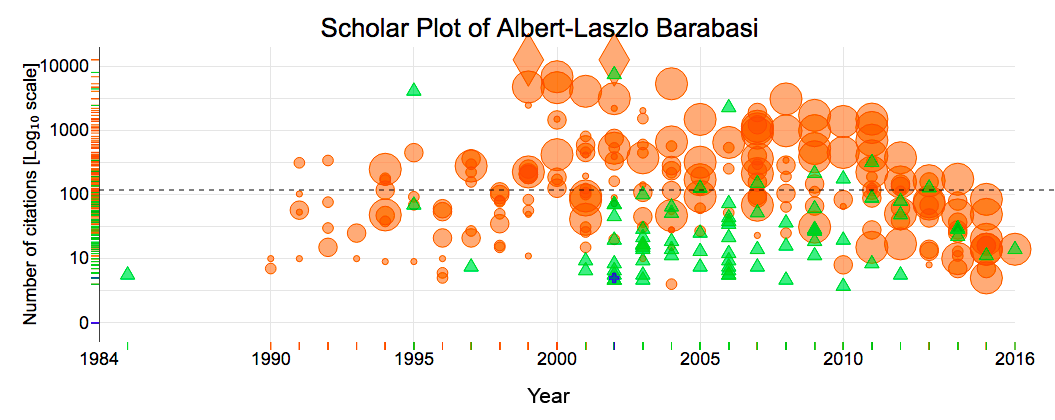
\includegraphics[width=.8\textwidth]{figures/fig_publication-3}
  \caption{An example of a famous physicist - Google Scholar Profile (Top) Curriculum Vitae (Middle) Scholar Plot (Bottom). Scholar Plot includes all the publications with different colors and symbols, which distinguish the type of publication.}~\label{fig-publication}
 % \vspace{-1ex}
\end{figure*}

% \begin{figure*}
%   \centering
%   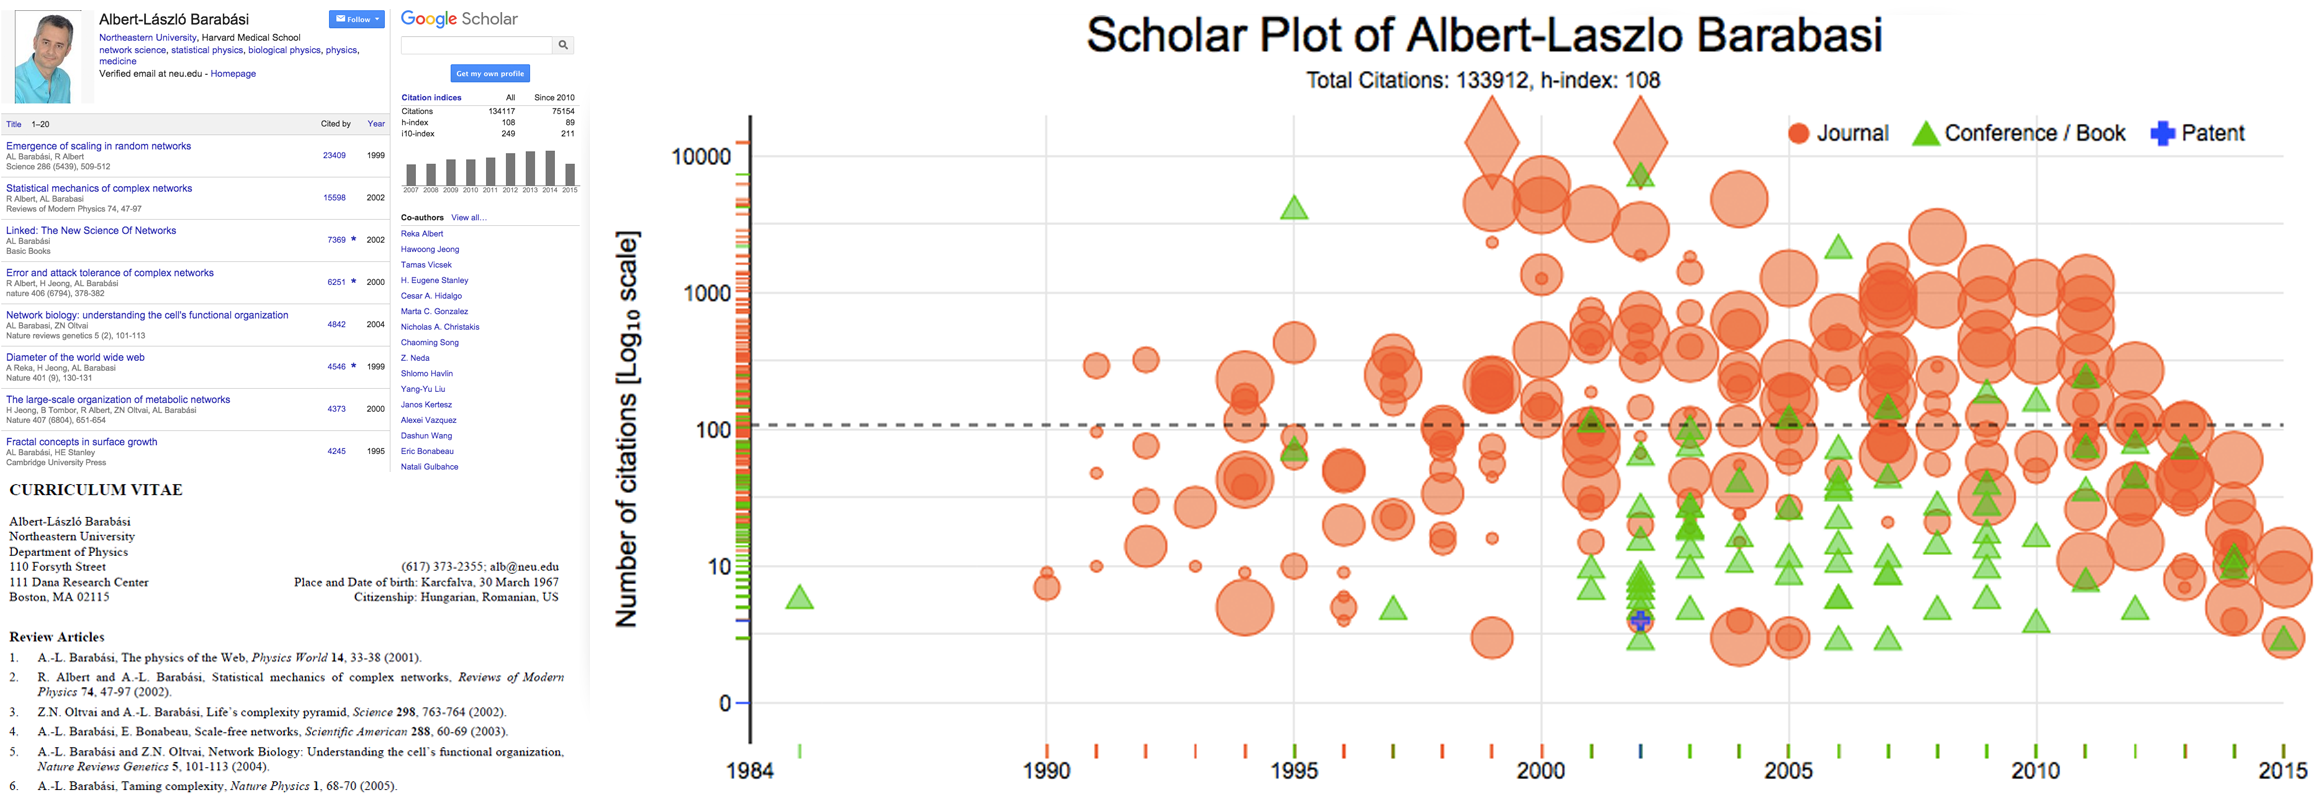
\includegraphics[width=1\textwidth]{figures/fig_cv_google_scholarplot}
%   \caption{An example of Scholar Plot - Visualizing Publication Data}~\label{fig-publication}
%  % \vspace{-1ex}
% \end{figure*}

Scholar Plot depicts the publications of an individual as a scatter plot and the NSF/NIH/NASA funding as a multiline plot. The publications are represented in a 2D diagram (number of citations vs. year of publication) with the {\it h}-index line. The horizontal axis is time, starting with the year of the researcher's first publication and ending with the current year. The vertical axis is the number of citations. The default plot is in $log_{10}$ scale. The user can also view the plot in the decimal scale by a toggle option using a radio button at the top left corner (Figure \ref{fig-scale}). The log scale provides a standardized scale that helps to compare the plots of multiple scholars.



% --------------------------
\subsection{Publication Data}
% --------------------------
Each publication is represented with a $i$ symbol. The center of the symbol has coordinates $(i_{PY}, i_{C})$, where $PY$ stands for Publication Year and $C$ for Number of citations obtained by the publication date. The journals are represented as circles (orange) with area analogous to the impact factor the journal, and the conferences / books are represented as triangles (green) and the patents as crosses (blue).

\begin{figure*}
    \centering
    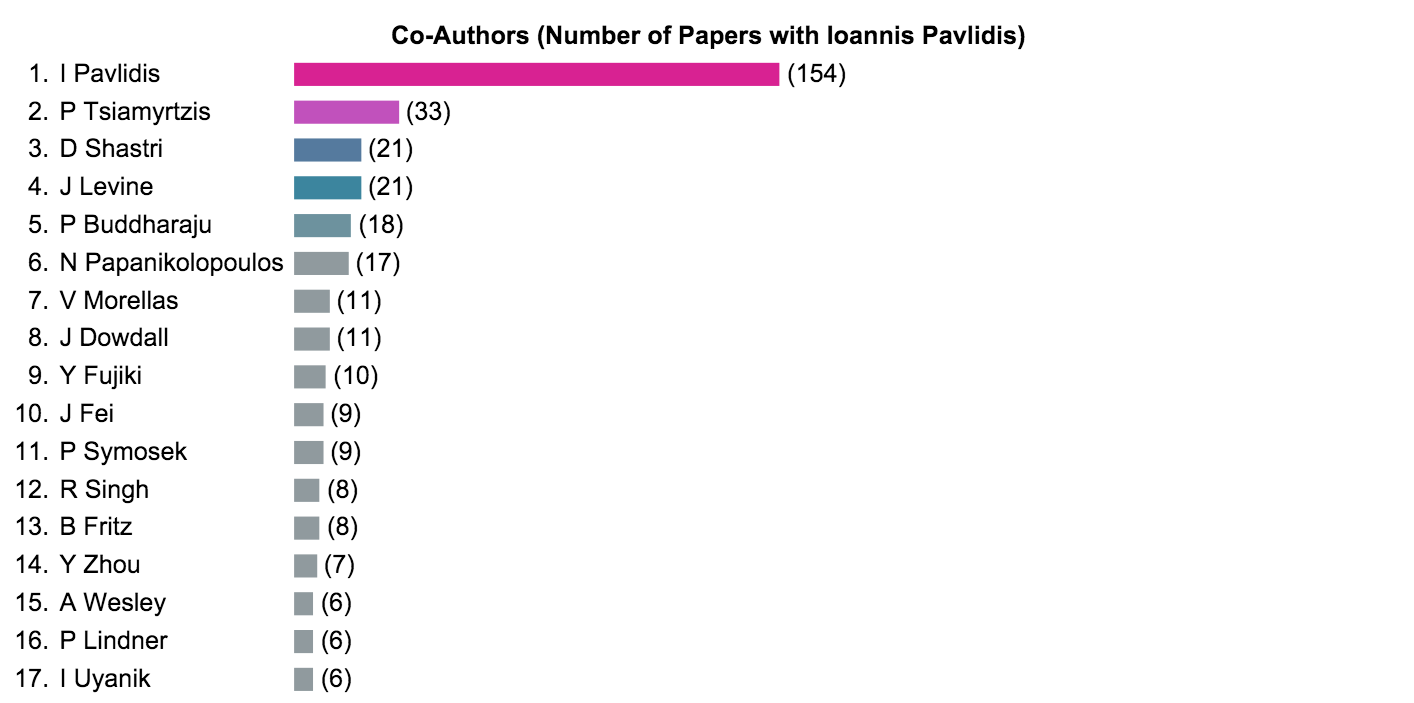
\includegraphics[width=1\textwidth]{figures/fig-panel-coauthros.png}
    \caption{The coauthor panel displays the author list.}~\label{fig-coauthors}
\end{figure*}

By clicking at a symbol, you can obtain the publication title, year, number of citations, the venue where published, and its impact factor (if it is a journal), as well as the breakdown in the authorship, complete with the level of collaboration between the co-authors and the selected scholar (Figure \ref{fig-tooltip}). The publication title also enables the user to navigate to the Google Scholar page for the selected paper. This helps to quickly verify and obtain further details of the selected publication. It allows users to access the PDF file directly, if available. To improve the user experience, I customized the tooltip to give detailed information without overlapping the plots.

\begin{figure}[H]
\centering
  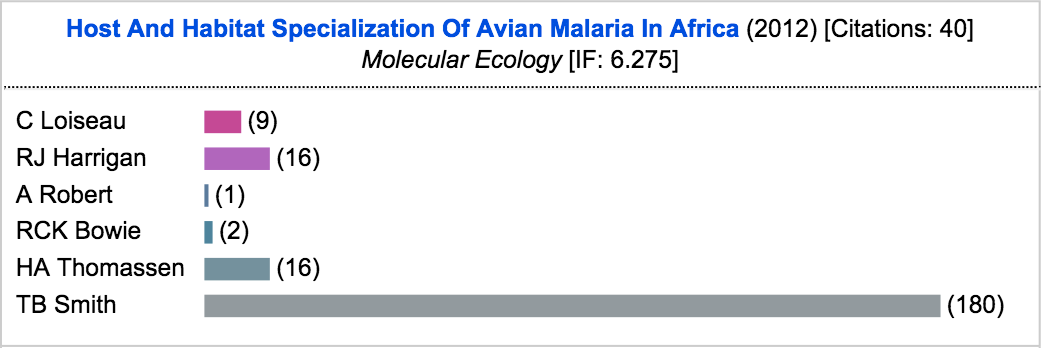
\includegraphics[width=1\textwidth]{figures/fig_tooltip}
  \caption{An example of the tooltip: the publication title, the year, the number of citations, the venue where published, impact factor, the list of co-authors, the visual horizontal bars with the number of collaboration between the co-authors, and the selected scholar.}~\label{fig-tooltip}
 % \vspace{-1ex}
\end{figure}

The dotted horizontal line on the plot denotes the {\it h}-index of the scholar as seen in Figures \ref{fig-scale}. Also, I denote the publications that earned greater than 10,000 citations with diamonds, as they represent the great success in publications (Figure \ref{fig-publication}). The title of the plot contains the name of the scholar and her/his total number of citations along with the {\it h}-index. At the top right corner, I display a legend distinguishing between the three different types of publications (Figure \ref{fig-legend}).

\begin{figure}[!htb]
\centering
  
\includegraphics[width=0.8\textwidth]{figures/fig_legend-toggle}
  \caption{The legend allows users to selectively view journals, conferences / books, and patents.}~\label{fig-legend}
 % \vspace{-1ex}
\end{figure}



I improved the user experience to enable users to quickly find and select from a pre-populated list of scholar names as they type. For each character the user enters, scholar plot displays similar matching names on the dropdown list. Even entering the space (`` "), it displays the 10 most recently inserted scholar's names. Scholar Plot follows the approach of responsive web design to provide optimal viewing based on the size of screen.



To place the plots in the personal Curriculum Vitae or on a personal web page, I developed the function in server-side, and provided a download button at the top right corner of the plot. This function enables the user to download plots in a zip file. It includes high resolution vector images in SVG (Scalable Vector Graphics) format of the publication and funding plots.






%% --------------------------
\subsection*{Ranked Density of Publication Types}
%% --------------------------
Scholar Plot also has a projection of the data on the y-axis depicted by small horizontal colored lines. For example, one can clearly see by the different colors that journals contribute to the {\it h}-index of the scholar in Figure \ref{fig:distribution} (a) and conferences / books contribute to the {\it h}-index of the scholar in Figure \ref{fig:distribution} (b). I conclude that the scholar in Figure \ref{fig:distribution} (c)) has many patents and the number of publications within a particular range of citations based on the density of the projected lines.

\begin{figure}[!htb]
\centering
\subfigure[]{%
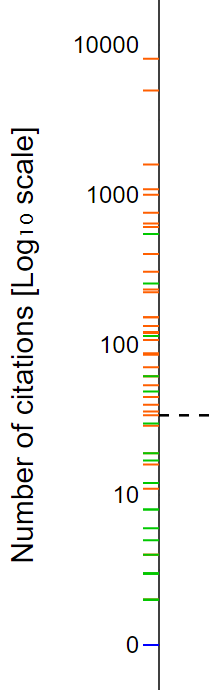
\includegraphics[width=0.23\textwidth]{figures/fig_distribution_A}
}
\subfigure[]{%
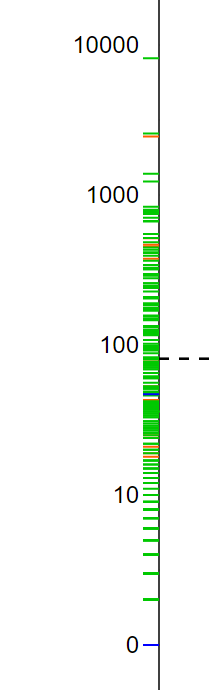
\includegraphics[width=0.23\textwidth]{figures/fig_distribution_B}
}
\subfigure[]{%
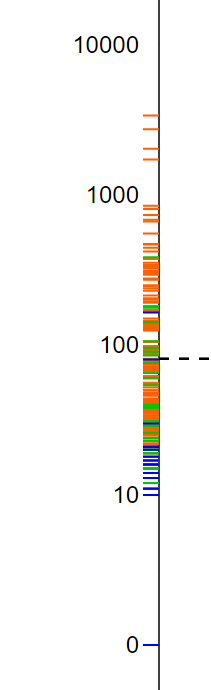
\includegraphics[width=0.23\textwidth]{figures/fig_distribution_C}
}
\caption{Examples of y-axis projection for three different scholars.}~\label{fig:distribution}
  %\vspace{-1ex}
\end{figure}

% \begin{figure}[!htb]
%  \centering
%  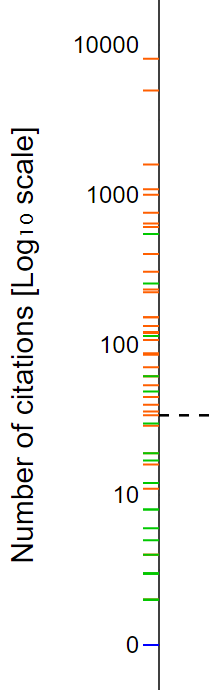
\includegraphics[width=0.2\textwidth]{figures/fig_distribution_A}
%  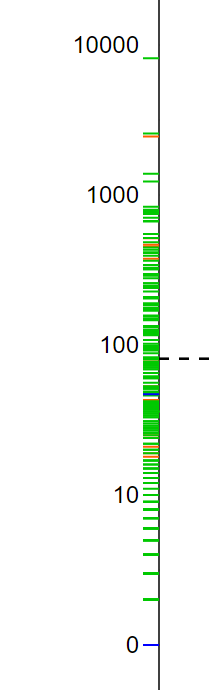
\includegraphics[width=0.2\textwidth]{figures/fig_distribution_B}
%  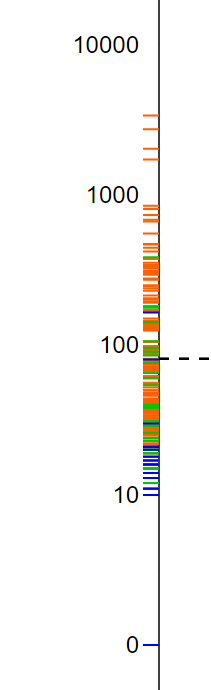
\includegraphics[width=0.2\textwidth]{figures/fig_distribution_C}
%  \caption{Example with journals, conferences, and patents contributing to h-index}~\label{fig:distribution}
% \end{figure}


Scholar plot brings different patterns of scholarly profiles. There are three types of patterns and each example as seen in Figures \ref{fig-RolandGlowinski}, \ref{fig-DannyReinberg}, and \ref{fig-ThadStarner}.


\begin{figure}%[!htb]
\centering
  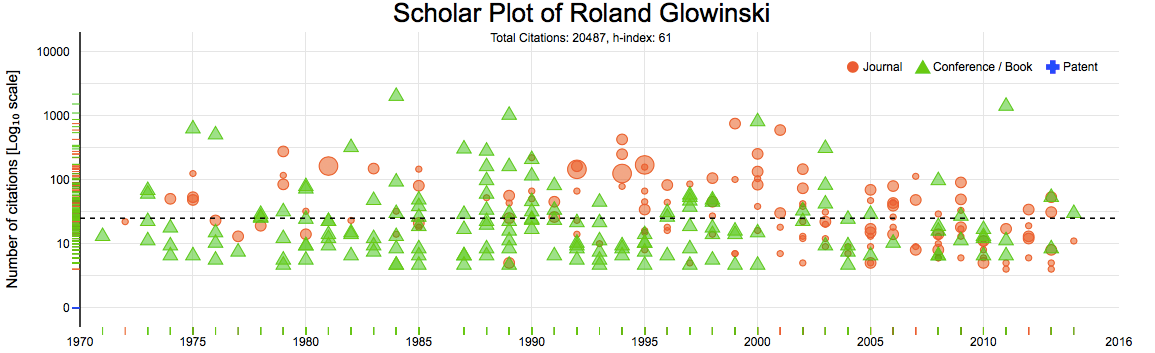
\includegraphics[width=1\textwidth]{figures/fig-RolandGlowinski}
  \caption{Examples of different scholarly profiles - Combination of journal and conference papers.}~\label{fig-RolandGlowinski}
\end{figure}

\begin{figure}%[!htb]
\centering
  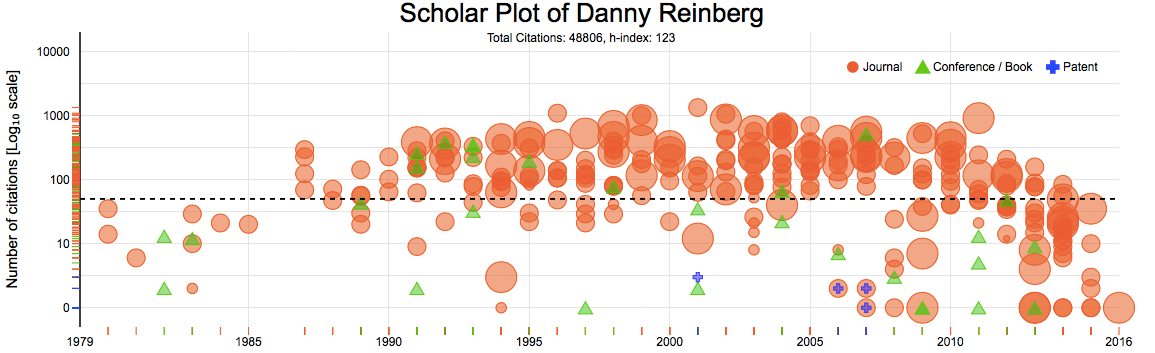
\includegraphics[width=1\textwidth]{figures/fig-DannyReinberg}
  \caption{Examples of different scholarly profiles - Preponderance of journal papers.}~\label{fig-DannyReinberg}
\end{figure}

\begin{figure}%[!htb]
\centering
  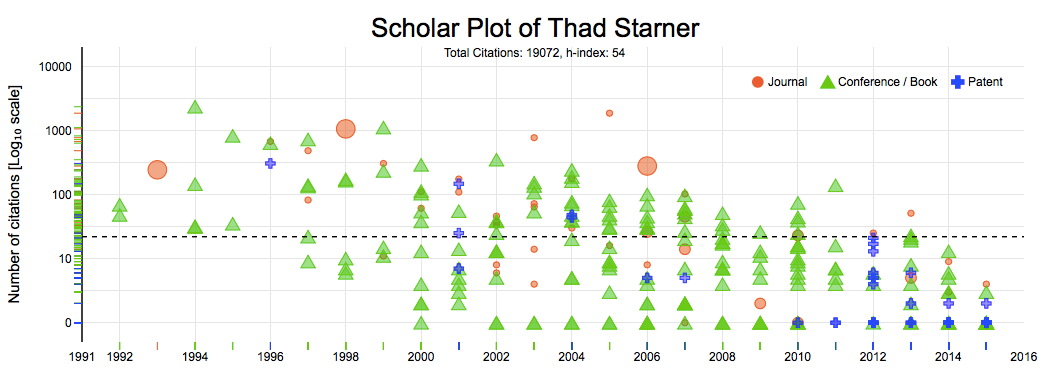
\includegraphics[width=1\textwidth]{figures/fig-ThadStarner}
  \caption{Examples of different scholarly profiles - Combination of conference papers and patents.}~\label{fig-ThadStarner}
\end{figure}






The user can bring the journals, patents, and conferences / books in and out of the view by clicking at the respective legend. If there is an overlap between journals, conferences, and patents, this feature can help the user to selectively view them. The user can also zoom the plot for a larger picture. Also, note that the symbols are not completely opaque. So if there are multiple symbols that overlap, the user can see and interact with them by hovering the mouse over them.


%% --------------------------
\subsection*{Disk Size - How to determine the size of disks}
%% --------------------------

\begin{figure*}
  \centering
  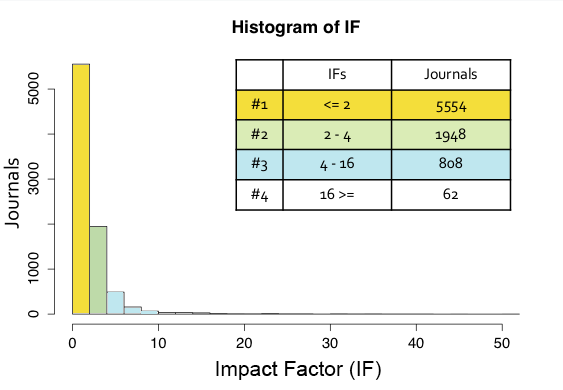
\includegraphics[width=0.7\textwidth]{figures/fig-Histogram-IF}
  \caption{Histogram of Impact Factor Jounal.}~\label{fig:Histogram-IF}
\end{figure*}

I wanted to plot a more efficient visual for journal publications, which is presented by different sizes, that tells the ranking of journal by Impact Factor Index. To do this, I analyzed the data set of JCR 2015 IF and ran a quartile function as a useful concept in statistics to determine the size of disks in Scholar Plot. Based on this number, the system will decide the size of the disk (Figure \ref{fig-disksize}) of each journal data and plot it in real-time. The quartile values are shown in Figure \ref{fig:Histogram-IF}. %The maximum number from descriptive is 153.459 through.

\begin{figure*}
  \centering
  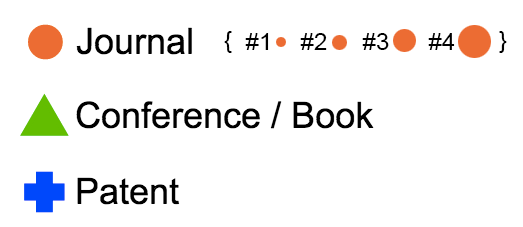
\includegraphics[width=0.5\textwidth]{figures/fig-disksize}
  \caption{Disk shapes and quartile sizes.}~\label{fig-disksize}
\end{figure*}





% --------------------------
\subsection{Funding Data}
% --------------------------
Scholar Plot also depicts the NSF/NIH/NASA funding of an individual as a multiline (Figure \ref{fig:funding}). Each breakpoint in the multiline corresponds to the individual's total amount in dollars of all NSF/NIH/NASA awards for the specific year. By pointing at a breakpoint you can obtain the NSF/NIH/NASA awards IDs, award amounts, and the investigator's role. The total annual funding information per year is also available by clicking the legend.

\begin{figure}[H]
  \centering
  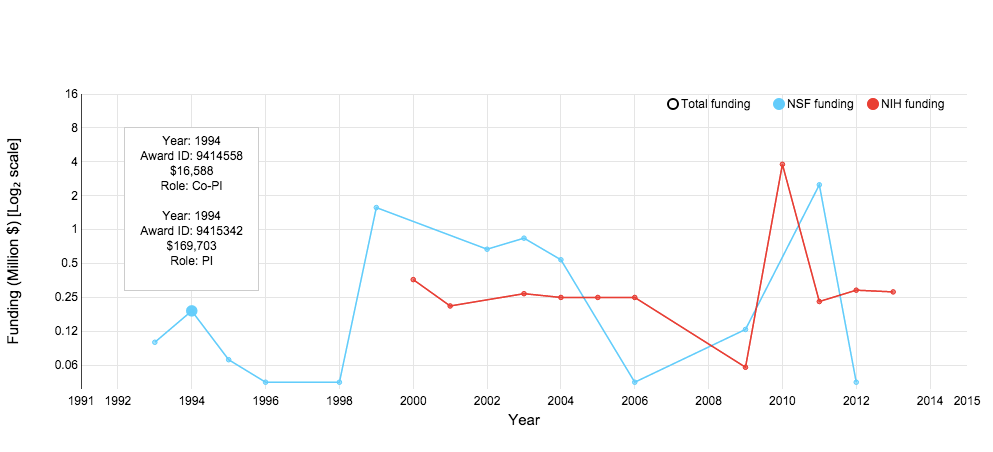
\includegraphics[width=1\textwidth]{figures/fig_funding_default}
  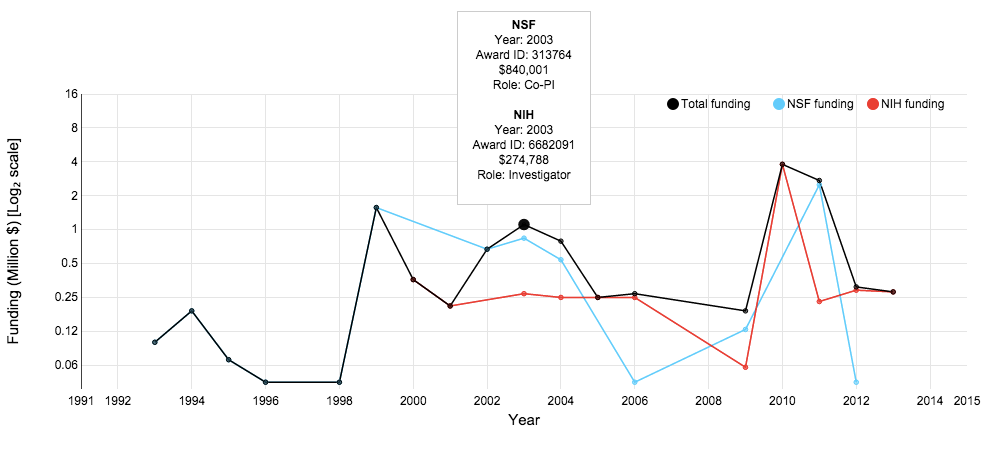
\includegraphics[width=1\textwidth]{figures/fig_funding_total}
  \caption{An example of Scholar Plot - Visualizing Funding Data.}~\label{fig:funding}
  % \vspace{-2ex}
\end{figure}






\begin{figure*}
    \centering
    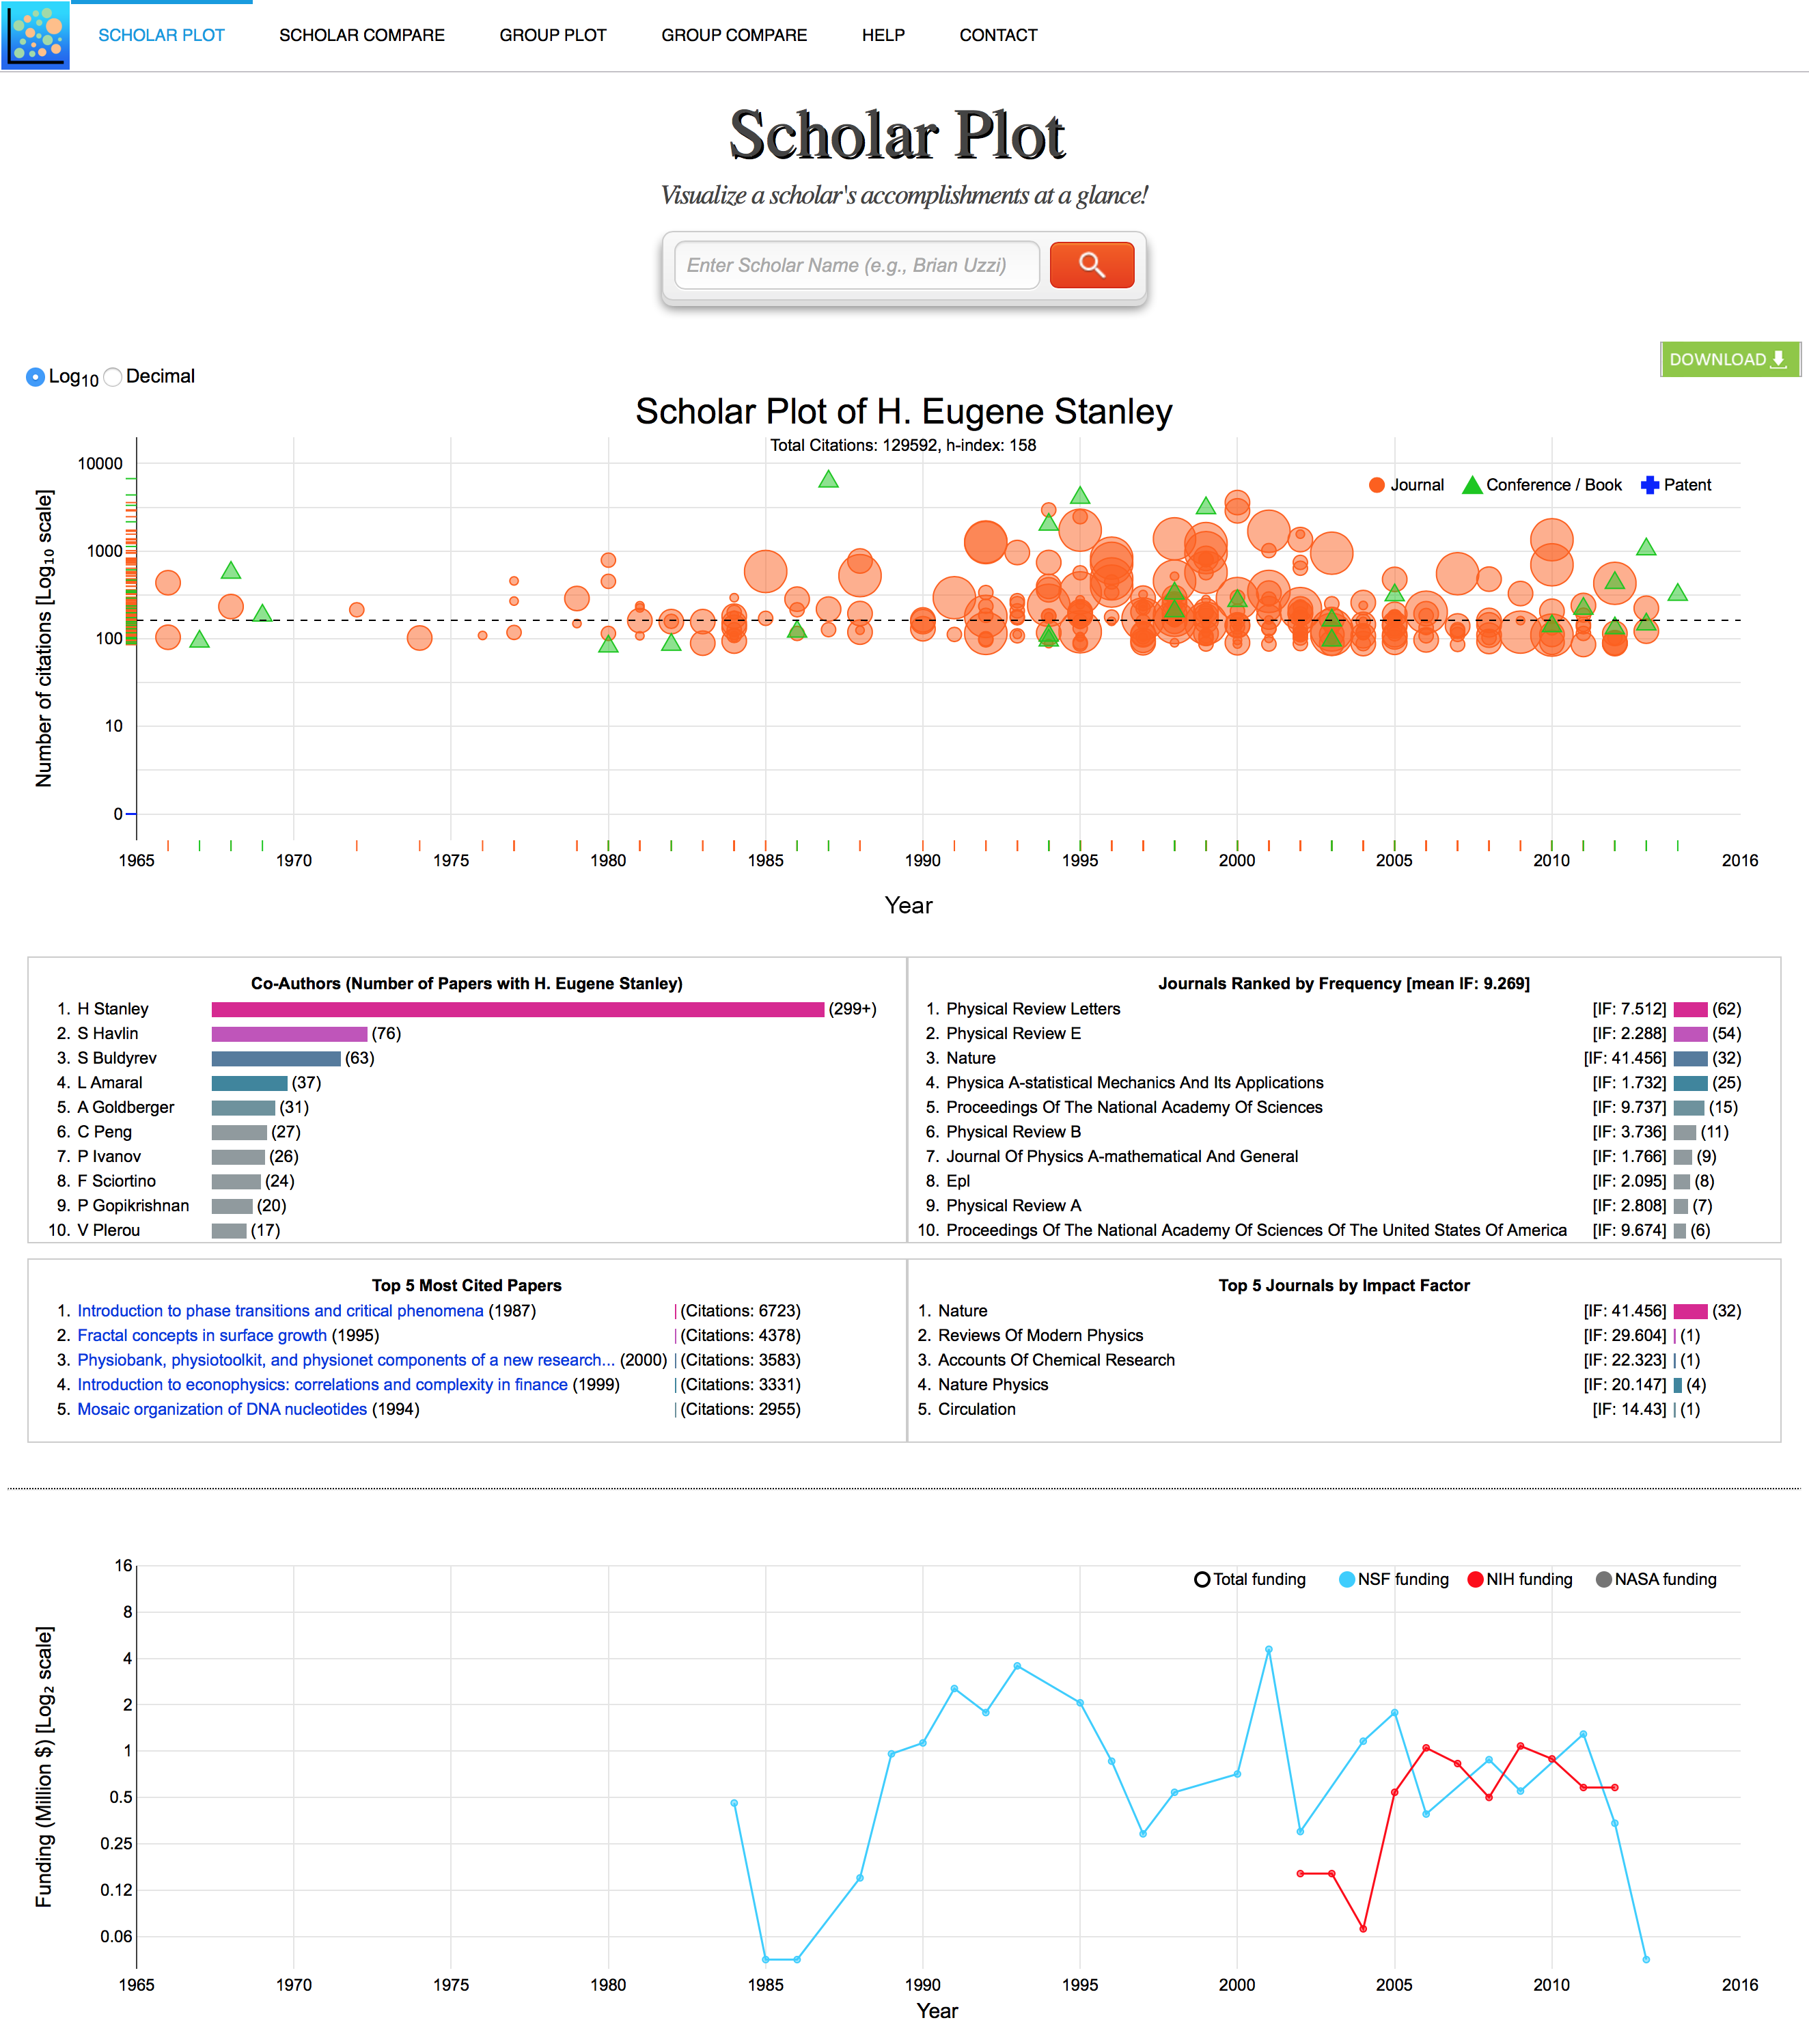
\includegraphics[width=1\textwidth]{figures/fig-Eugene-with-menu}
    \caption{Base level Scholar Plot (SP) example - a famous physicist and interdisciplinary scientist with dozens of articles in \emph{Nature}. The summary panels in the middle were added after a feedback from the focus group. Notice how this scholar's publication production exploded in sync with the commencement of substantial federal funding.}~\label{fig-scholarplot-full}
\end{figure*}





% --------------------------
\section{Department Plot - Group Visualization}
% --------------------------
The group level of Scholar Plot visualizes department/college academic records. One of the important issues was to determine how to scale the individual visualization to the group level. Group plot consists of 2 aspects - plot at the department level and at the college level. I applied our design philosophy at the group level. I use pie charts and bar charts to display the information in a compact manner. Pie charts are useful to show a proportion of contribution of each individual to the group (i.e. department). For pie-charts, I displayed the top 5 scholars to avoid overcrowding the pie chart.

%\begin{figure}[H]
%  \centering
%  \includegraphics[width=1\textwidth]{figures/fig-h-HD}
%  \caption{Example of bar chart by h-index.}~\label{fig:groupplot}
%\end{figure}

% --------------------------
\subsection{Department Plot}
% --------------------------

Departmental Plot is an attempt to visualize aspects of tenured and tenure-track faculty contributions to their home department. These aspects include intellectual contributions as well as non-intellectual factors such as funding. The faculty are compared based on publicly available measures like h-index, citations, and impact factor. I visualized a citation contribution as a pie chart normalized by the number of years in which a scholar spent in academia. Also, I portrayed charts depicting the highest (Home Run) cited paper and the highest (Home Run) impact factor journal where the scholar published.


\begin{figure*}
  \centering
  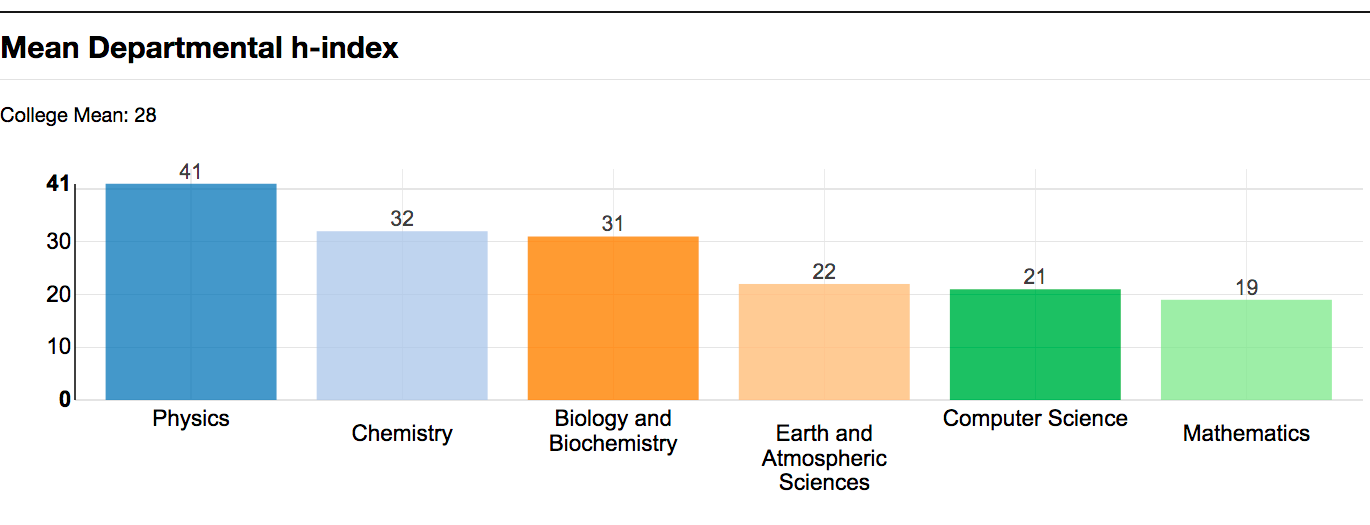
\includegraphics[width=1\textwidth]{figures/Coll-h-HD}
  \caption{Mean Departmental h-index
 - College of Natural Sciences and Mathematics at University of Houston.}~\label{fig:DP-College1}
\end{figure*}

\begin{figure*}
  \centering
  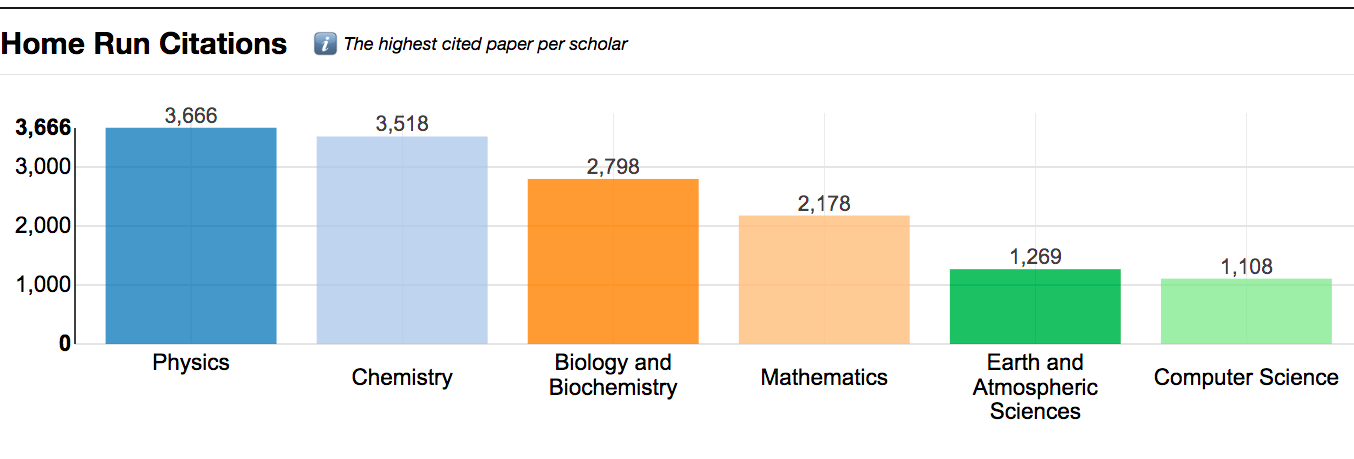
\includegraphics[width=1\textwidth]{figures/Coll-Cit-HD}
  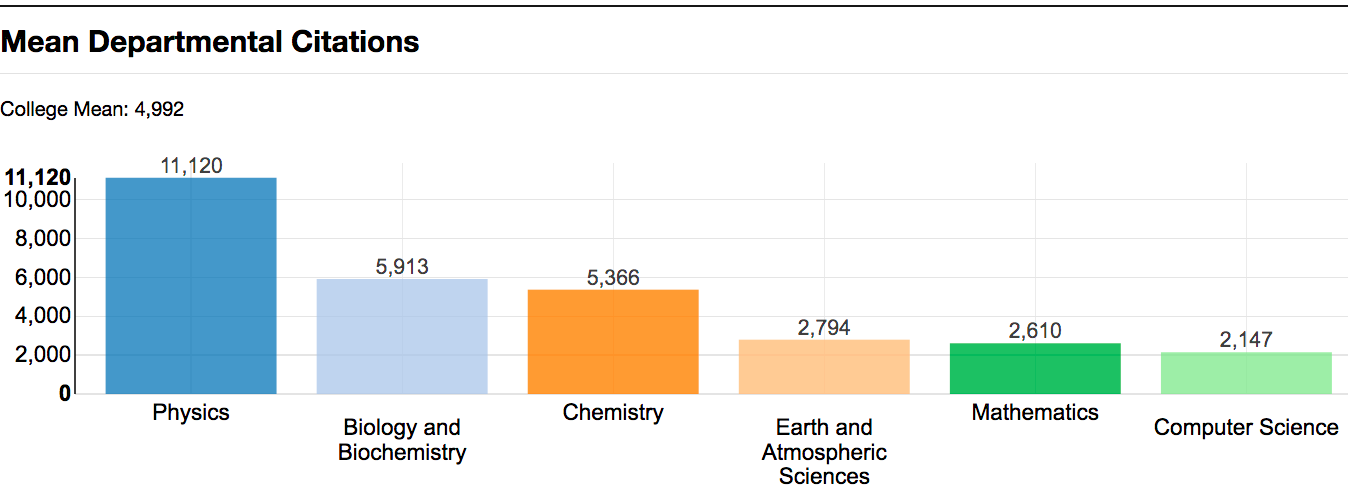
\includegraphics[width=1\textwidth]{figures/Coll-Cit-HD2}
  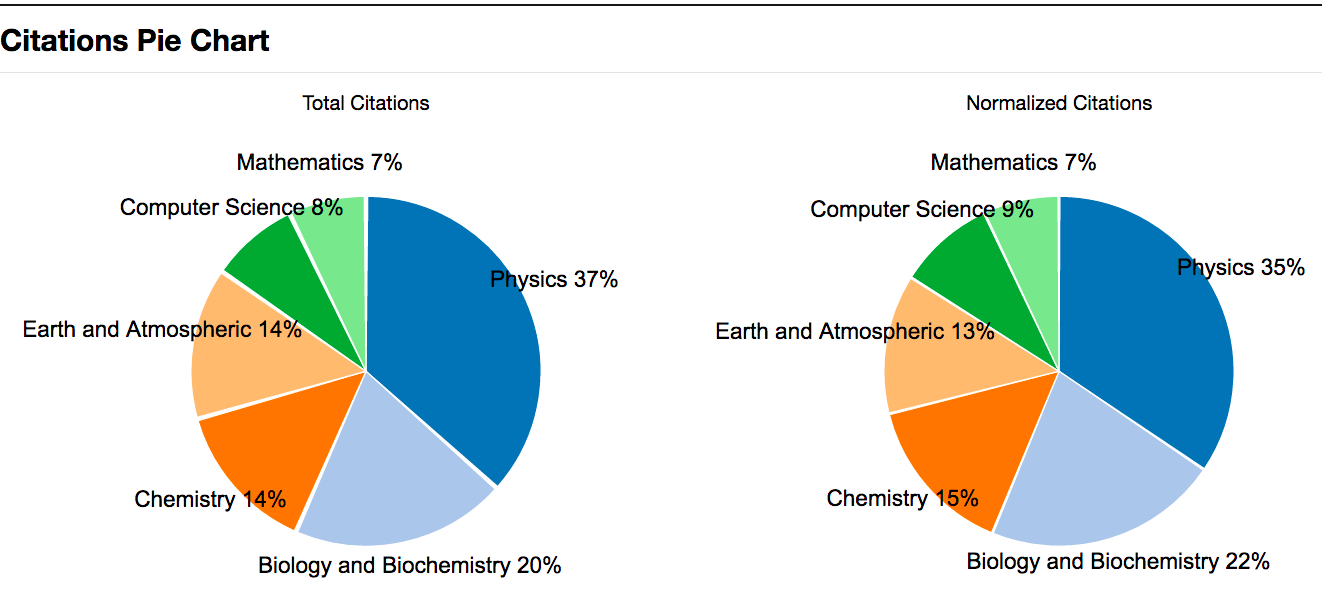
\includegraphics[width=1\textwidth]{figures/Coll-Cit-HD3}
  \caption{Home Run Citations, Mean Departmental Citations, and Citations Pie Chart (Total Citations and Normalized Citations) - College of Natural Sciences and Mathematics at University of Houston.}~\label{fig:DP-College1}
\end{figure*}

\begin{figure*}
  \centering
  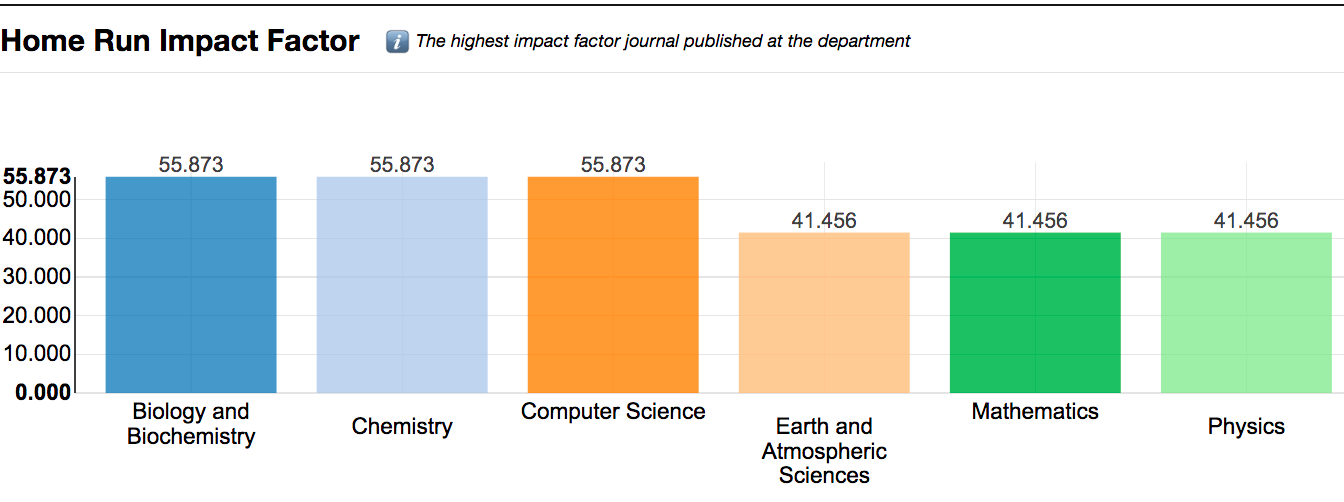
\includegraphics[width=1\textwidth]{figures/Coll-IF-HD}
  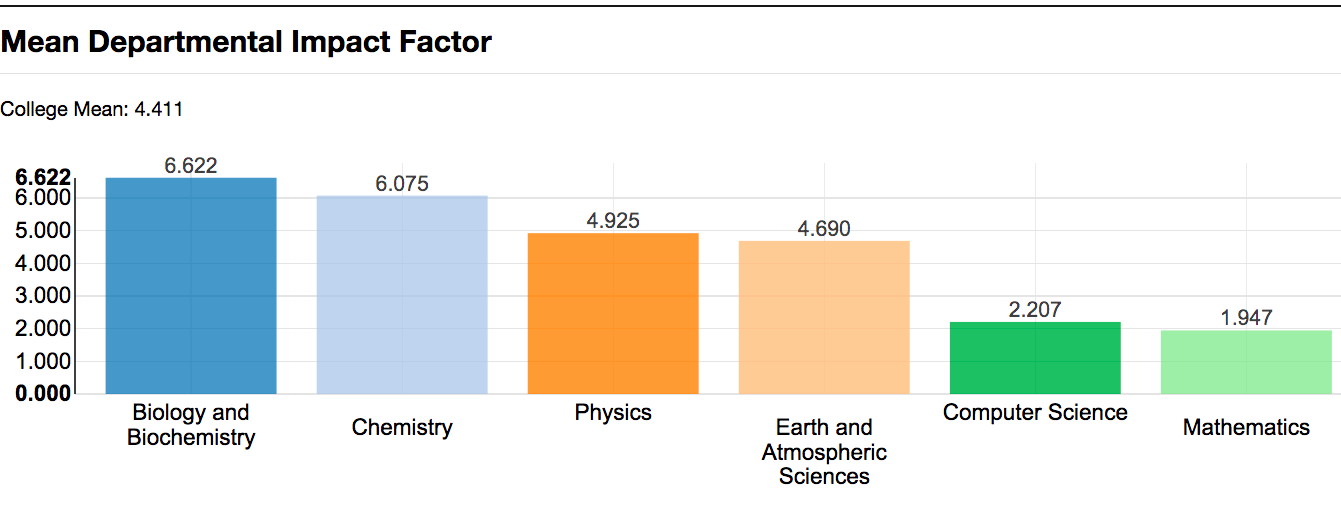
\includegraphics[width=1\textwidth]{figures/Coll-IF-HD2}
  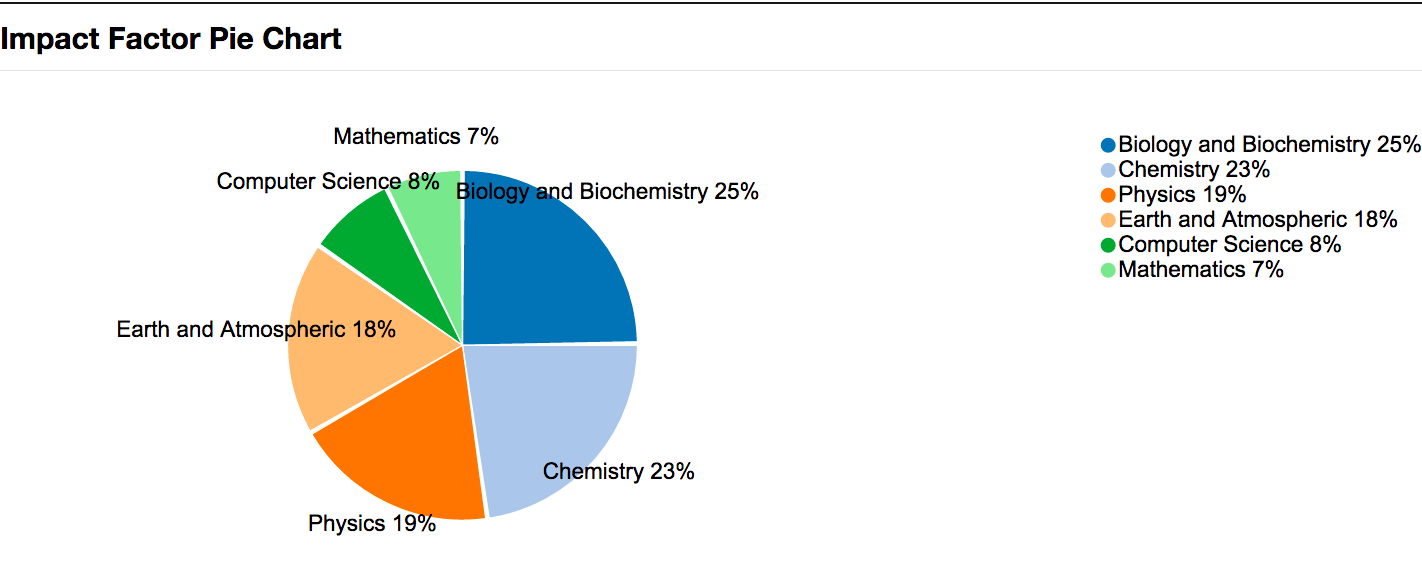
\includegraphics[width=1\textwidth]{figures/Coll-IF-HD3}
  \caption{Home Run Impact Factor, Mean Departmental Impact Factor, and Impact Factor Pie Chart - College of Natural Sciences and Mathematics at University of Houston.}~\label{fig:DP-College1}
\end{figure*}

\begin{figure*}
  \centering
  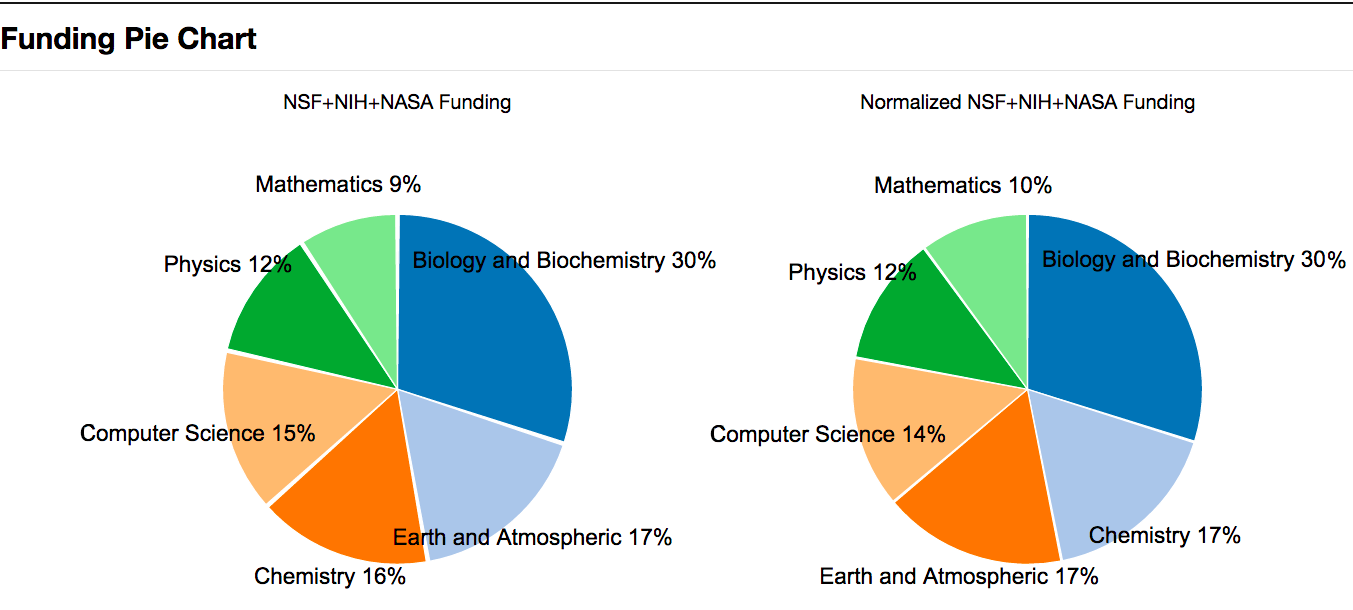
\includegraphics[width=1\textwidth]{figures/Coll-Fund-HD}
  \caption{Funding Pie Chart - College of Natural Sciences and Mathematics at University of Houston.}~\label{fig:DP-College1}
\end{figure*}


% ------------------------------------------------------------------
\subsection{Department Plot Glossary}
% ------------------------------------------------------------------

\begin{description}
  \item[H-INDEX] \hfill \\
  The h-index is a form of measure that takes into account the number of citations and number of total publications made by a scholar.
  \item[HOME RUN CITATIONS] \hfill \\
  The Home Run Citations bar chart shows the highest cited paper within the department, with the largest number of citations of a publication on the y-axis, and the scholar associated with that publication on the x-axis.
  \item[CITATIONS] \hfill \\
  The Citations bar chart displays the total amount of citations a scholar has received through all of his/her publications.
  \item[CITATIONS PIE CHART] \hfill \\
  The Citations Pie Chart displays the percentage of citations that each scholar produced out of all the citations in the department.
  \item[HOME RUN IMPACT FACTOR] \hfill \\
  The Home Run Impact Factor bar chart shows the highest journal impact factor for each of the deparment's scholars. The impact factor is on the y-axis and the name of the scholar is on the x-axis.
  \item[MEAN IMPACT FACTOR] \hfill \\
  The Mean Impact Factor bar chart shows the average level of journal impact factor by each scholar in the department with the impact factor on the y-axis and the name of the scholar on the x-axis.
  \item[IMPACT FACTOR PIE CHART] \hfill \\
  The Impact Factor Pie Chart displays the percentage of journal impact that each scholar is responsible for out of the total journal impact of the college.
  \item[FUNDING] \hfill \\
  The funding bar chart shows the amount of funding awarded to each scholars in the department with the amount of dollars in funding on the y-axis and the scholar associated with that funding on the x-axis.
  \item[FUNDING PIE CHART] \hfill \\
  The Funding Pie Chart displays the percentage of funding that each scholar has received in the department.
\end{description}




% --------------------------
\subsection{College Plot}
% --------------------------

College plot attempts to visualize the contributions of the departments to the home college. College plot pictures the mean values of various measures described above for each department. I used pie charts and bar charts like in the department plot. Note that the data for department and college plot is generated by using a query to our database.


\begin{figure*}
  \centering
  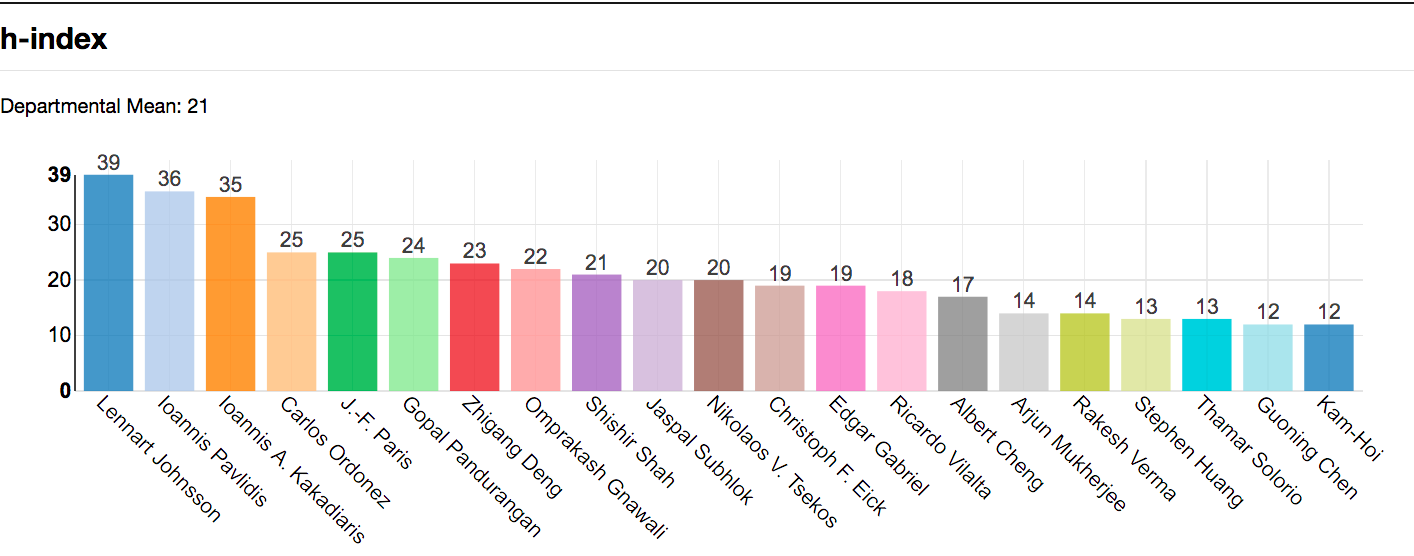
\includegraphics[width=1\textwidth]{figures/Dept-h-HD}
  \caption{hIndex - Department of Computer Science at University of Houston.}~\label{fig:DP-College1}
\end{figure*}

\begin{figure*}
  \centering
  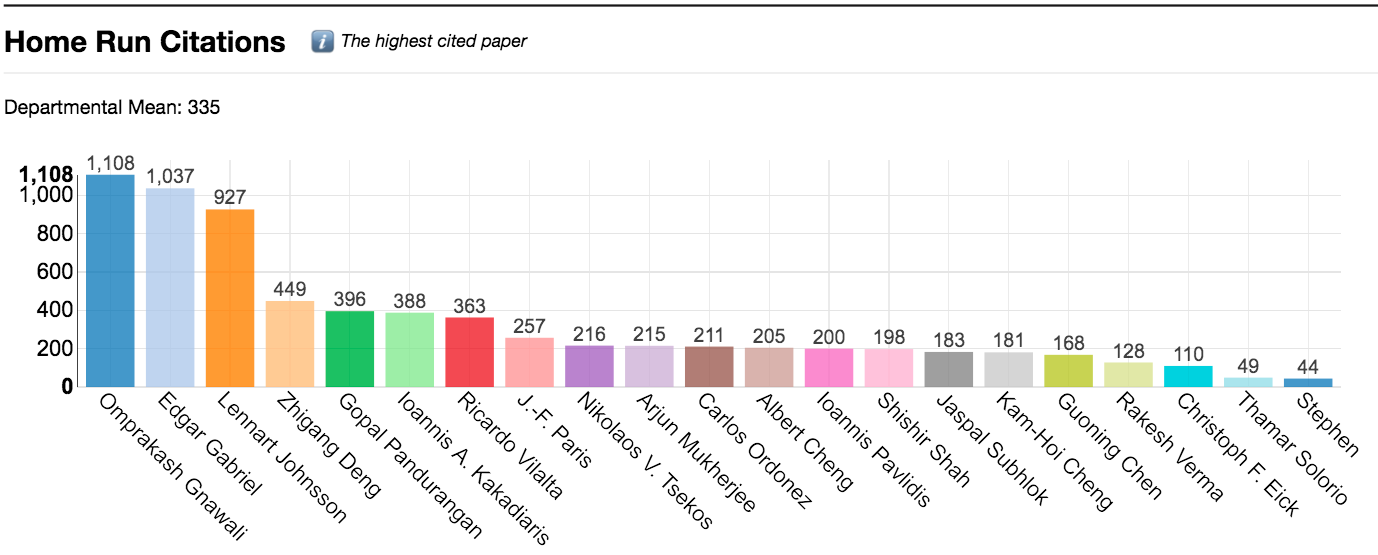
\includegraphics[width=1\textwidth]{figures/Dept-Cit-HD}
  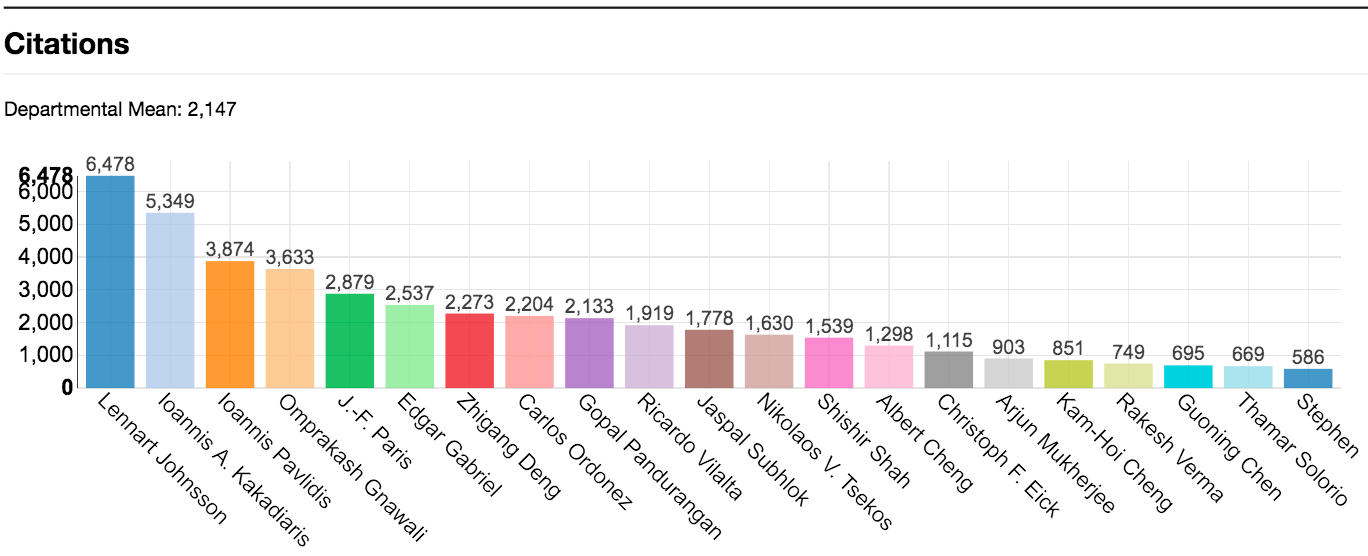
\includegraphics[width=1\textwidth]{figures/Dept-Cit-HD2}
  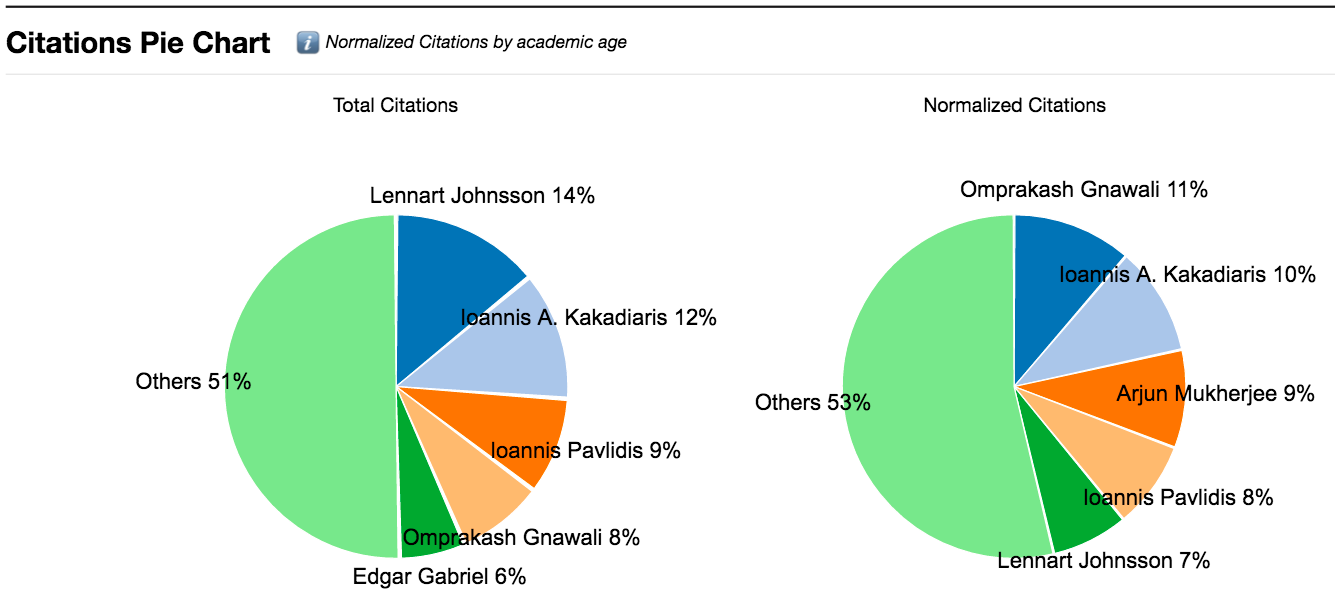
\includegraphics[width=1\textwidth]{figures/Dept-Cit-HD3}
 
  \caption{Home Run Citations, Citations, and Citations Pie Chart (Total Citations, Normalized Citations) - Department of Computer Science at University of Houston - Citation.}~\label{fig:DP-College1}
\end{figure*}

\begin{figure*}
  \centering
  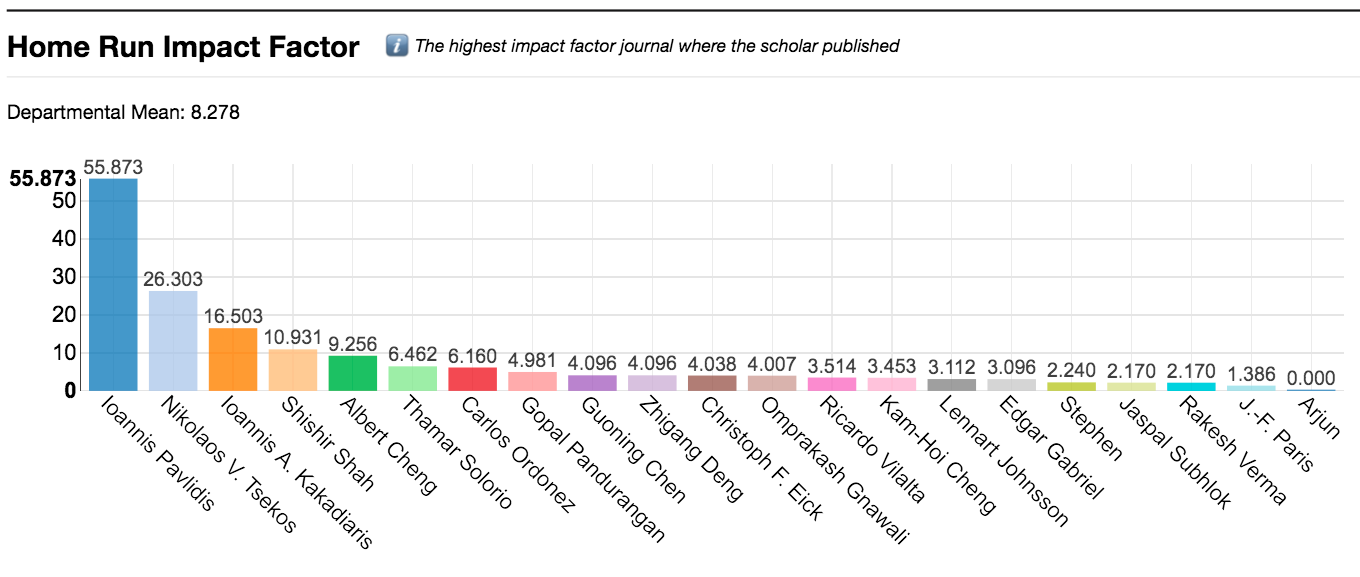
\includegraphics[width=1\textwidth]{figures/Dept-IF-HD}
  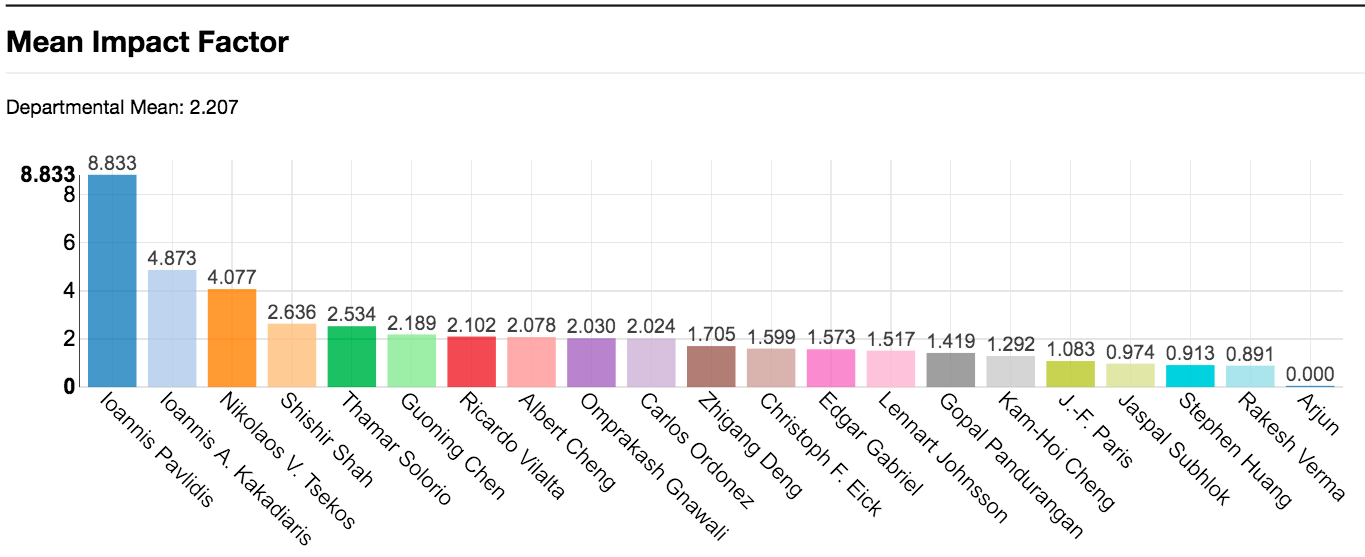
\includegraphics[width=1\textwidth]{figures/Dept-IF-HD2}
  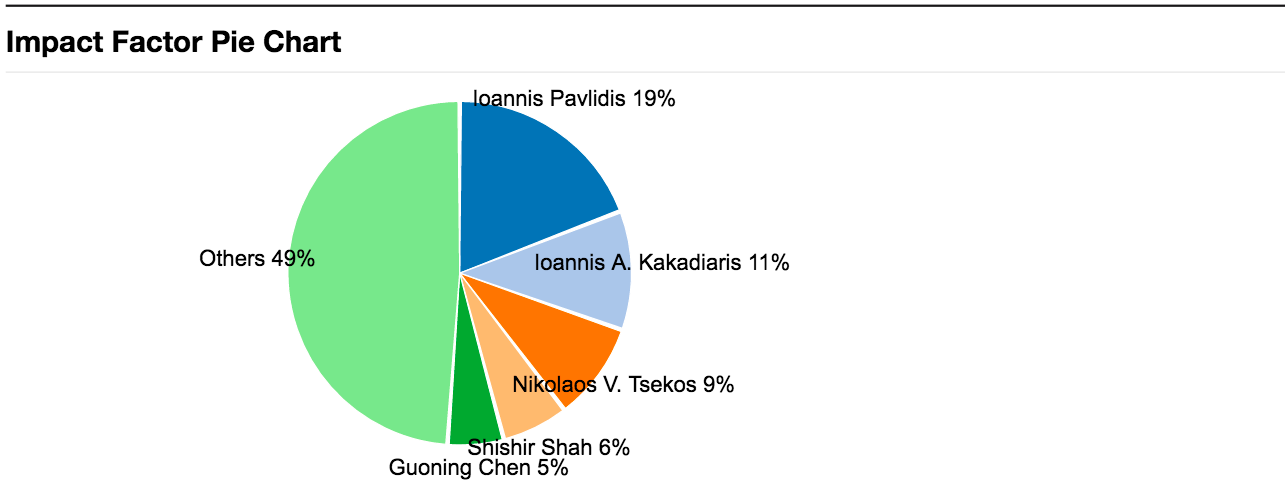
\includegraphics[width=1\textwidth]{figures/Dept-IF-HD3}
  \caption{Home Run Impact Factor, Mean Impact Factor, and Impact Factor Pie Chart - Department of Computer Science at University of Houston - Impact Factor.}~\label{fig:DP-College1}
\end{figure*}

\begin{figure*}
  \centering
  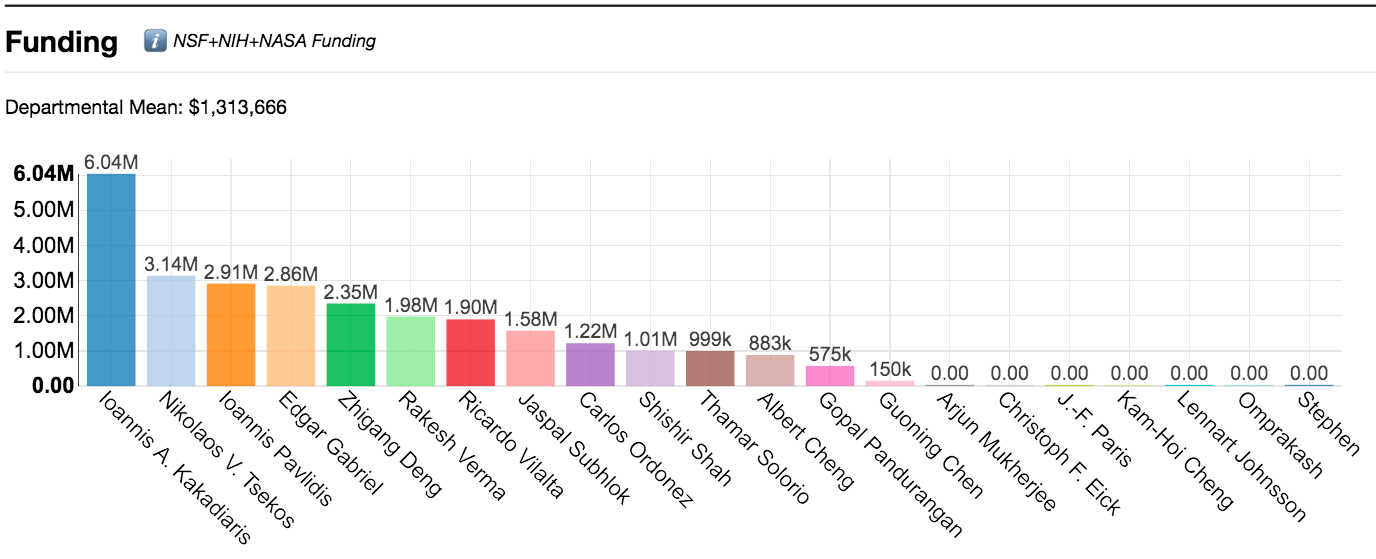
\includegraphics[width=1\textwidth]{figures/Dept-Fund-HD}
  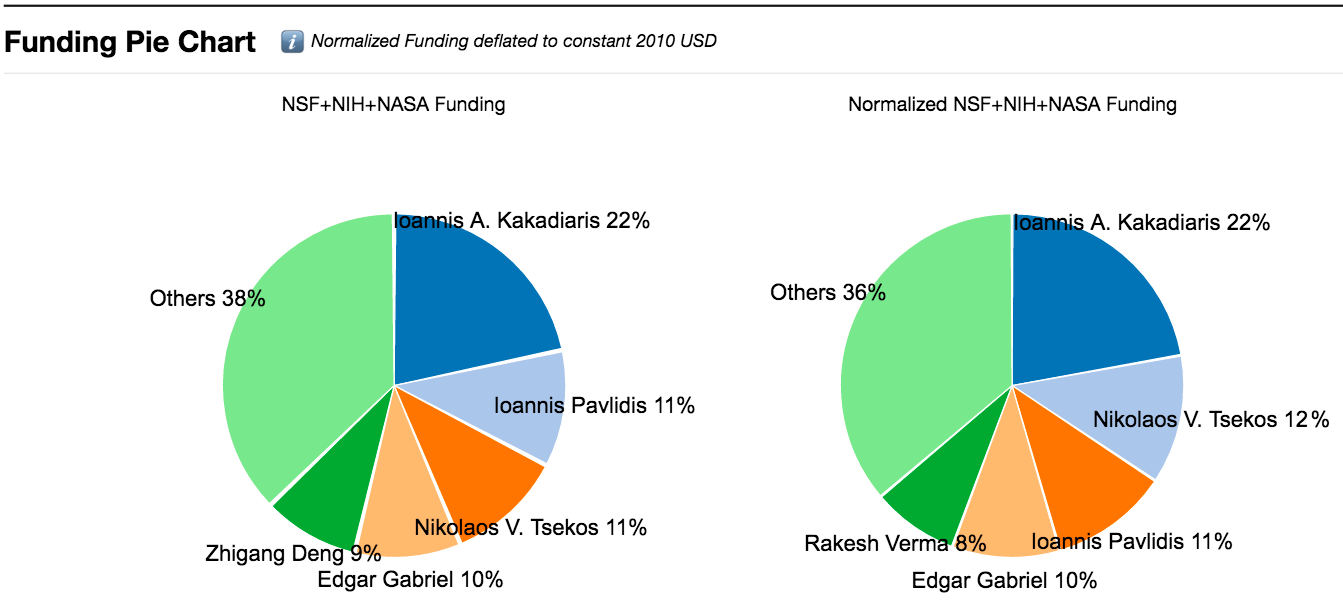
\includegraphics[width=1\textwidth]{figures/Dept-Fund-HD2}
  \caption{Funding, Funding Pie Chart (NSF+NIH+NASA Funding, Normalized NSF+NIH+NASA Funding) - Department of Computer Science at University of Houston - Funding.}~\label{fig:DP-College1}
\end{figure*}






% ------------------------------------------------------------------
\subsection{College Plot Glossary}
% ------------------------------------------------------------------



\begin{description}
  \item[FUNDING PIE CHART] \hfill \\
  The Funding Pie Chart displays the percentage of funding that each scholar has received in the department.
  \item[MEAN DEPARTMENTAL H-INDEX] \hfill \\
  The Mean Departmental h-index bar chart shows the average h-index for each department in the selected college. The y-axis is the mean h-index and the x-axis is the department name.
  \item[HOME RUN CITATIONS] \hfill \\
  The Home Run Citations bar chart shows the number of citations of the highest cited paper within each department on the y-axis and the names of the departments on the x-axis.
  \item[MEAN DEPARTMENTAL CITATIONS] \hfill \\
  The Mean Departmental Citations bar chart shows the average number of citations for the scholars in each department with the number of citations on the y-axis and the names of the departments on the x-axis.
  \item[CITATIONS PIE CHART] \hfill \\
  The Home Run Impact Factor bar chart shows the highest journal impact factor of each department with the impact factor on the y-axis and the names of the departments on the x-axis.
  \item[HOME RUN IMPACT FACTOR] \hfill \\
  The Citations Pie Chart displays the percentage of citations that each department produced out of all the citations in the college.
  \item[MEAN DEPARTMENTAL IMPACT FACTOR] \hfill \\
  The Mean Department Impact Factor bar chart shows the average level of journal impact factor by each department with the impact factor on the y-axis and the department on the x-axis.
  \item[IMPACT FACTOR PIE CHART] \hfill \\
  The Impact Factor Pie Chart displays the percentage of journal impact that each department is responsible for out of the total journal impact of the college.
  \item[FUNDING PIE CHART] \hfill \\
  The Funding Pie Chart displays the percentage of funding that each department has received in the college.
\end{description}




% --------------------------
\subsection{Compare Plot}
% --------------------------




%\begin{figure*}
%  \centering
%  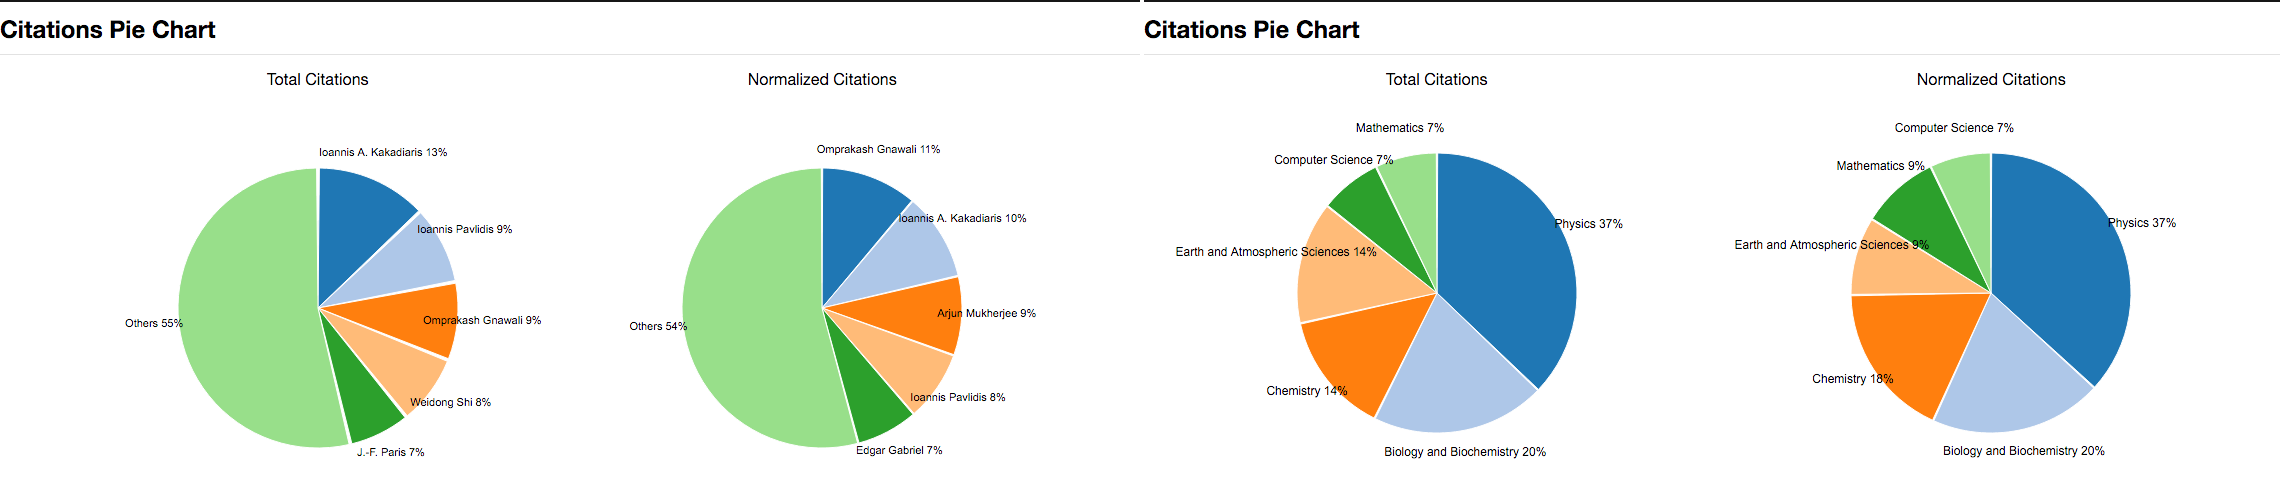
\includegraphics[width=1\textwidth]{figures/fig-Group-Citation}
%  \caption{Example of Citations Pie Chart. The ones on the left are at the Department Level, the ones on right are at the College Level. The charts depict total citations and normalized citations.}~\label{fig:Group-Cit}
%\end{figure*}




Department Compare aims to assist people to have a deeper understanding of the inner accomplishments in the departments. It complements the ranking given to the department by the US News Report. Department Compare feature compares the departments with the same publicly available measures. Scholar plot compares the summary statistics like the mean values. It uses box plots to compare the distribution of values of the individual faculty in each department. To determine whether a result is statistically significant, box plots denote the significant sign.

\begin{figure*}
  \centering
  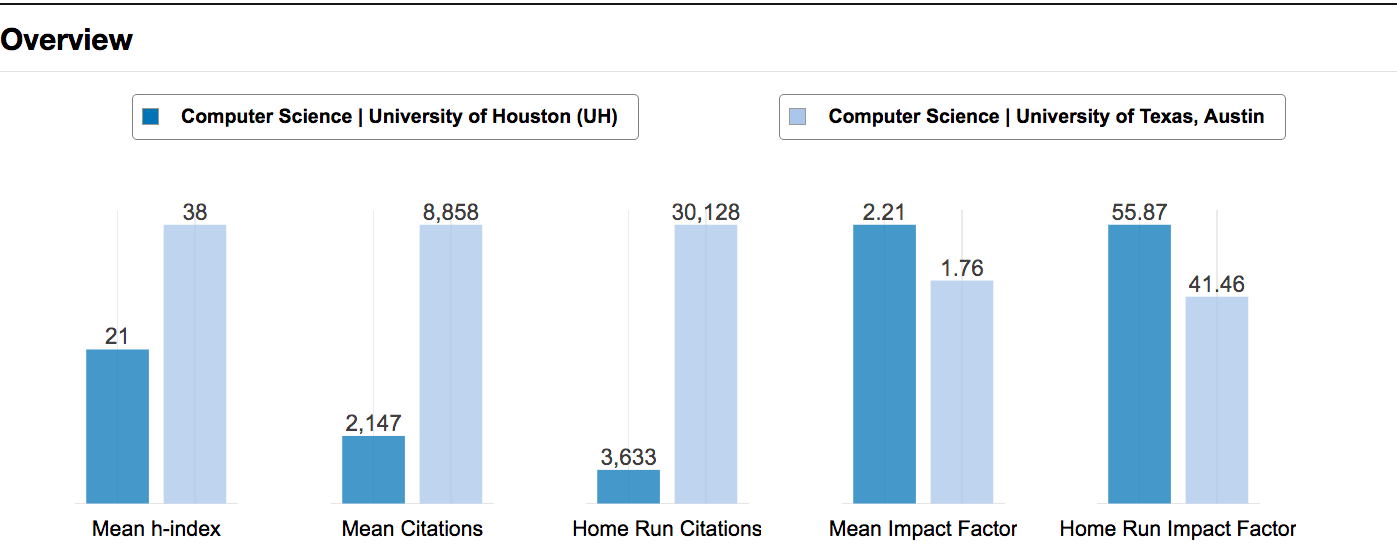
\includegraphics[width=1\textwidth]{figures/fig-GroupCompare-HD}
  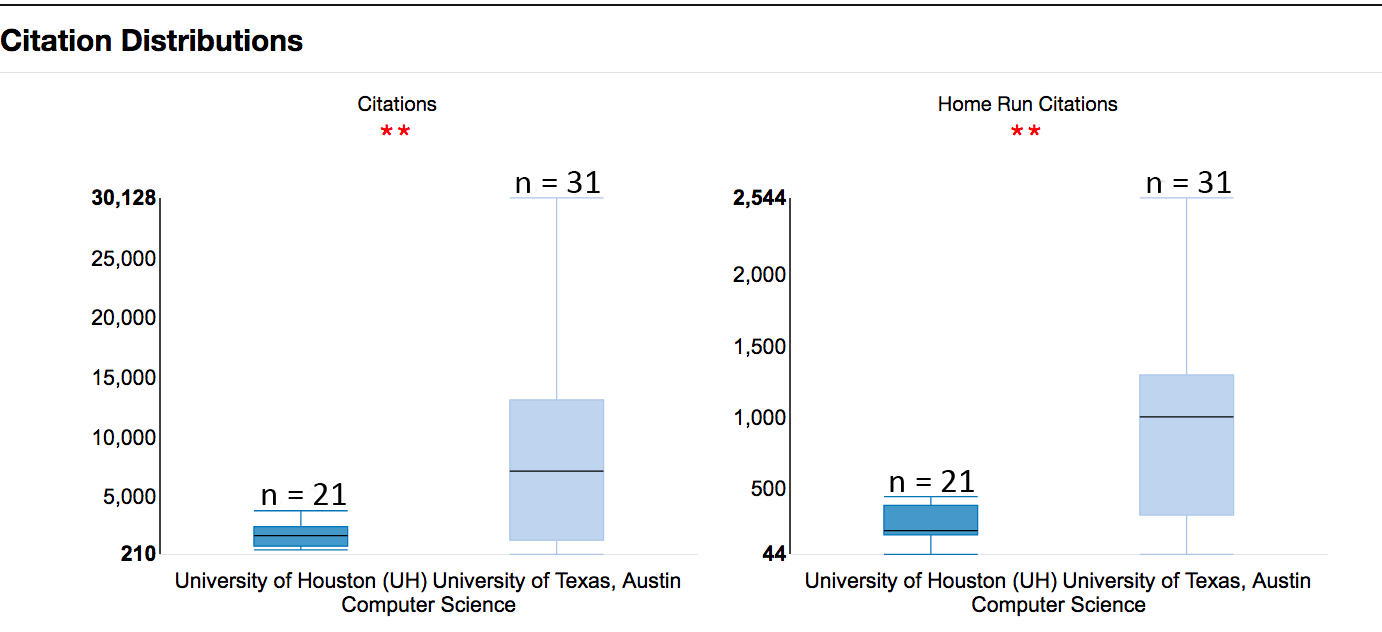
\includegraphics[width=1\textwidth]{figures/fig-GroupCompare-HD2}
  \caption{Example of Group Compare between Departments of Computer Science at University of Houston and the University of Texas - Austin.}~\label{fig:groupcompare}
\end{figure*}







% ------------------------------------------------------------------
\subsection{Compare Plot Glossary}
% ------------------------------------------------------------------




\begin{description}
  \item[OVERVIEW] \hfill \\
  The overview displays the mean h-index, mean citations, and home run citations for the two departments in the form of multiple bar graphs. Each color represents one of the departments, indicated by the key at the top of the section.
  \item[H-INDEX DISTRIBUTIONS] \hfill \\
  The h-index distributions chart displays the spread of the h-indexes within a department through box plots. The n value above each box plot represents the sample size used. The stars below the title of each section signify the statistical significance.
  \item[CITATION DISTRIBUTIONS] \hfill \\
  The Citations Distributions chart shows the spread of the citations within the department for each university. The n value above each box plot represents the sample size used. The stars below the title of each section signify the statistical significance.
  \item[IMPACT FACTOR DISTRIBUTIONS] \hfill \\
  The Impact Factor Distributions chart displays the spread of citations within a department through box plots. The n value above each box plot represents the sample size used. The stars below the title of each section signify the statistical significance.
\end{description}












% ==================================================
  % \chapter{Academic Garden}\label{chap:Academic Garden}
% ==================================================
% ------------------------------------------------------------------
\section {Academic Garden - Scalable Visualization}
% ------------------------------------------------------------------
Academic Garden (AG) is a scalable visualization of academic merit. It applies to individual academics, departments, colleges, and any other academic group thereof, such as a research lab or a project team. Reminiscent of the legal views for physical personhood and corporate personhood, we consider that individual academics and academic groups share behavioral characteristics. Specifically, we argue that academic performance has three pillars that are scale invariant: (a) funding that enables intellectual production; (b) prestige of the venues where intellectual products appear; and, (c) impact of the intellectual products. In the case of groups, these three variables are expressed as statistics of the corresponding individual measurements. 

Academic Garden uses the flower metaphor to visually articulate performance for academic entities. The width of the flower's stem is commensurate to the academic funding this entity received (`juice conduit'). The height of the flower's stem is commensurate to the impact of the entity's intellectual products (`visibility'). The diameter of the flower's disc is commensurate to the prestige of the venues where these products appeared (`fancy factor'). %As secondary characteristics, the number of petal colors is commensurate to the multi-disciplinarily of the entity's intellectual production with the bud vs. bloom appearance denotes the academic entity's age.




% ------------------------------------------------------------------
\subsection {Research Funding: Enabler of Production}
% ------------------------------------------------------------------
Research funding is an enabler of academic production. Very few things can be done in the absence of funding in science and engineering. Even in humanities, some funding is needed in many cases (e.g., travel support for archival research).  Research funding is dispensed through peer-reviewed proposal competitions, and for this reason, it is not only an enabler but also has inherent merit. As different disciplines need different levels of funding some normalization is in order. This normalization can be any statistic. We prefer the quartile where the funding level of the academic entity's record belongs with respect to all the records in the specific discipline.  `All' here is commensurate to the selected reference, whether this is a university department or a set of departments across the United States. Needless to say that the original funding records need to be adjusted, taking into account the entity's age (if the entity is a physical person) or the number of individuals participating in the entity's personhood (if the entity is a group). 

% \begin{figure*}
%     \centering
%     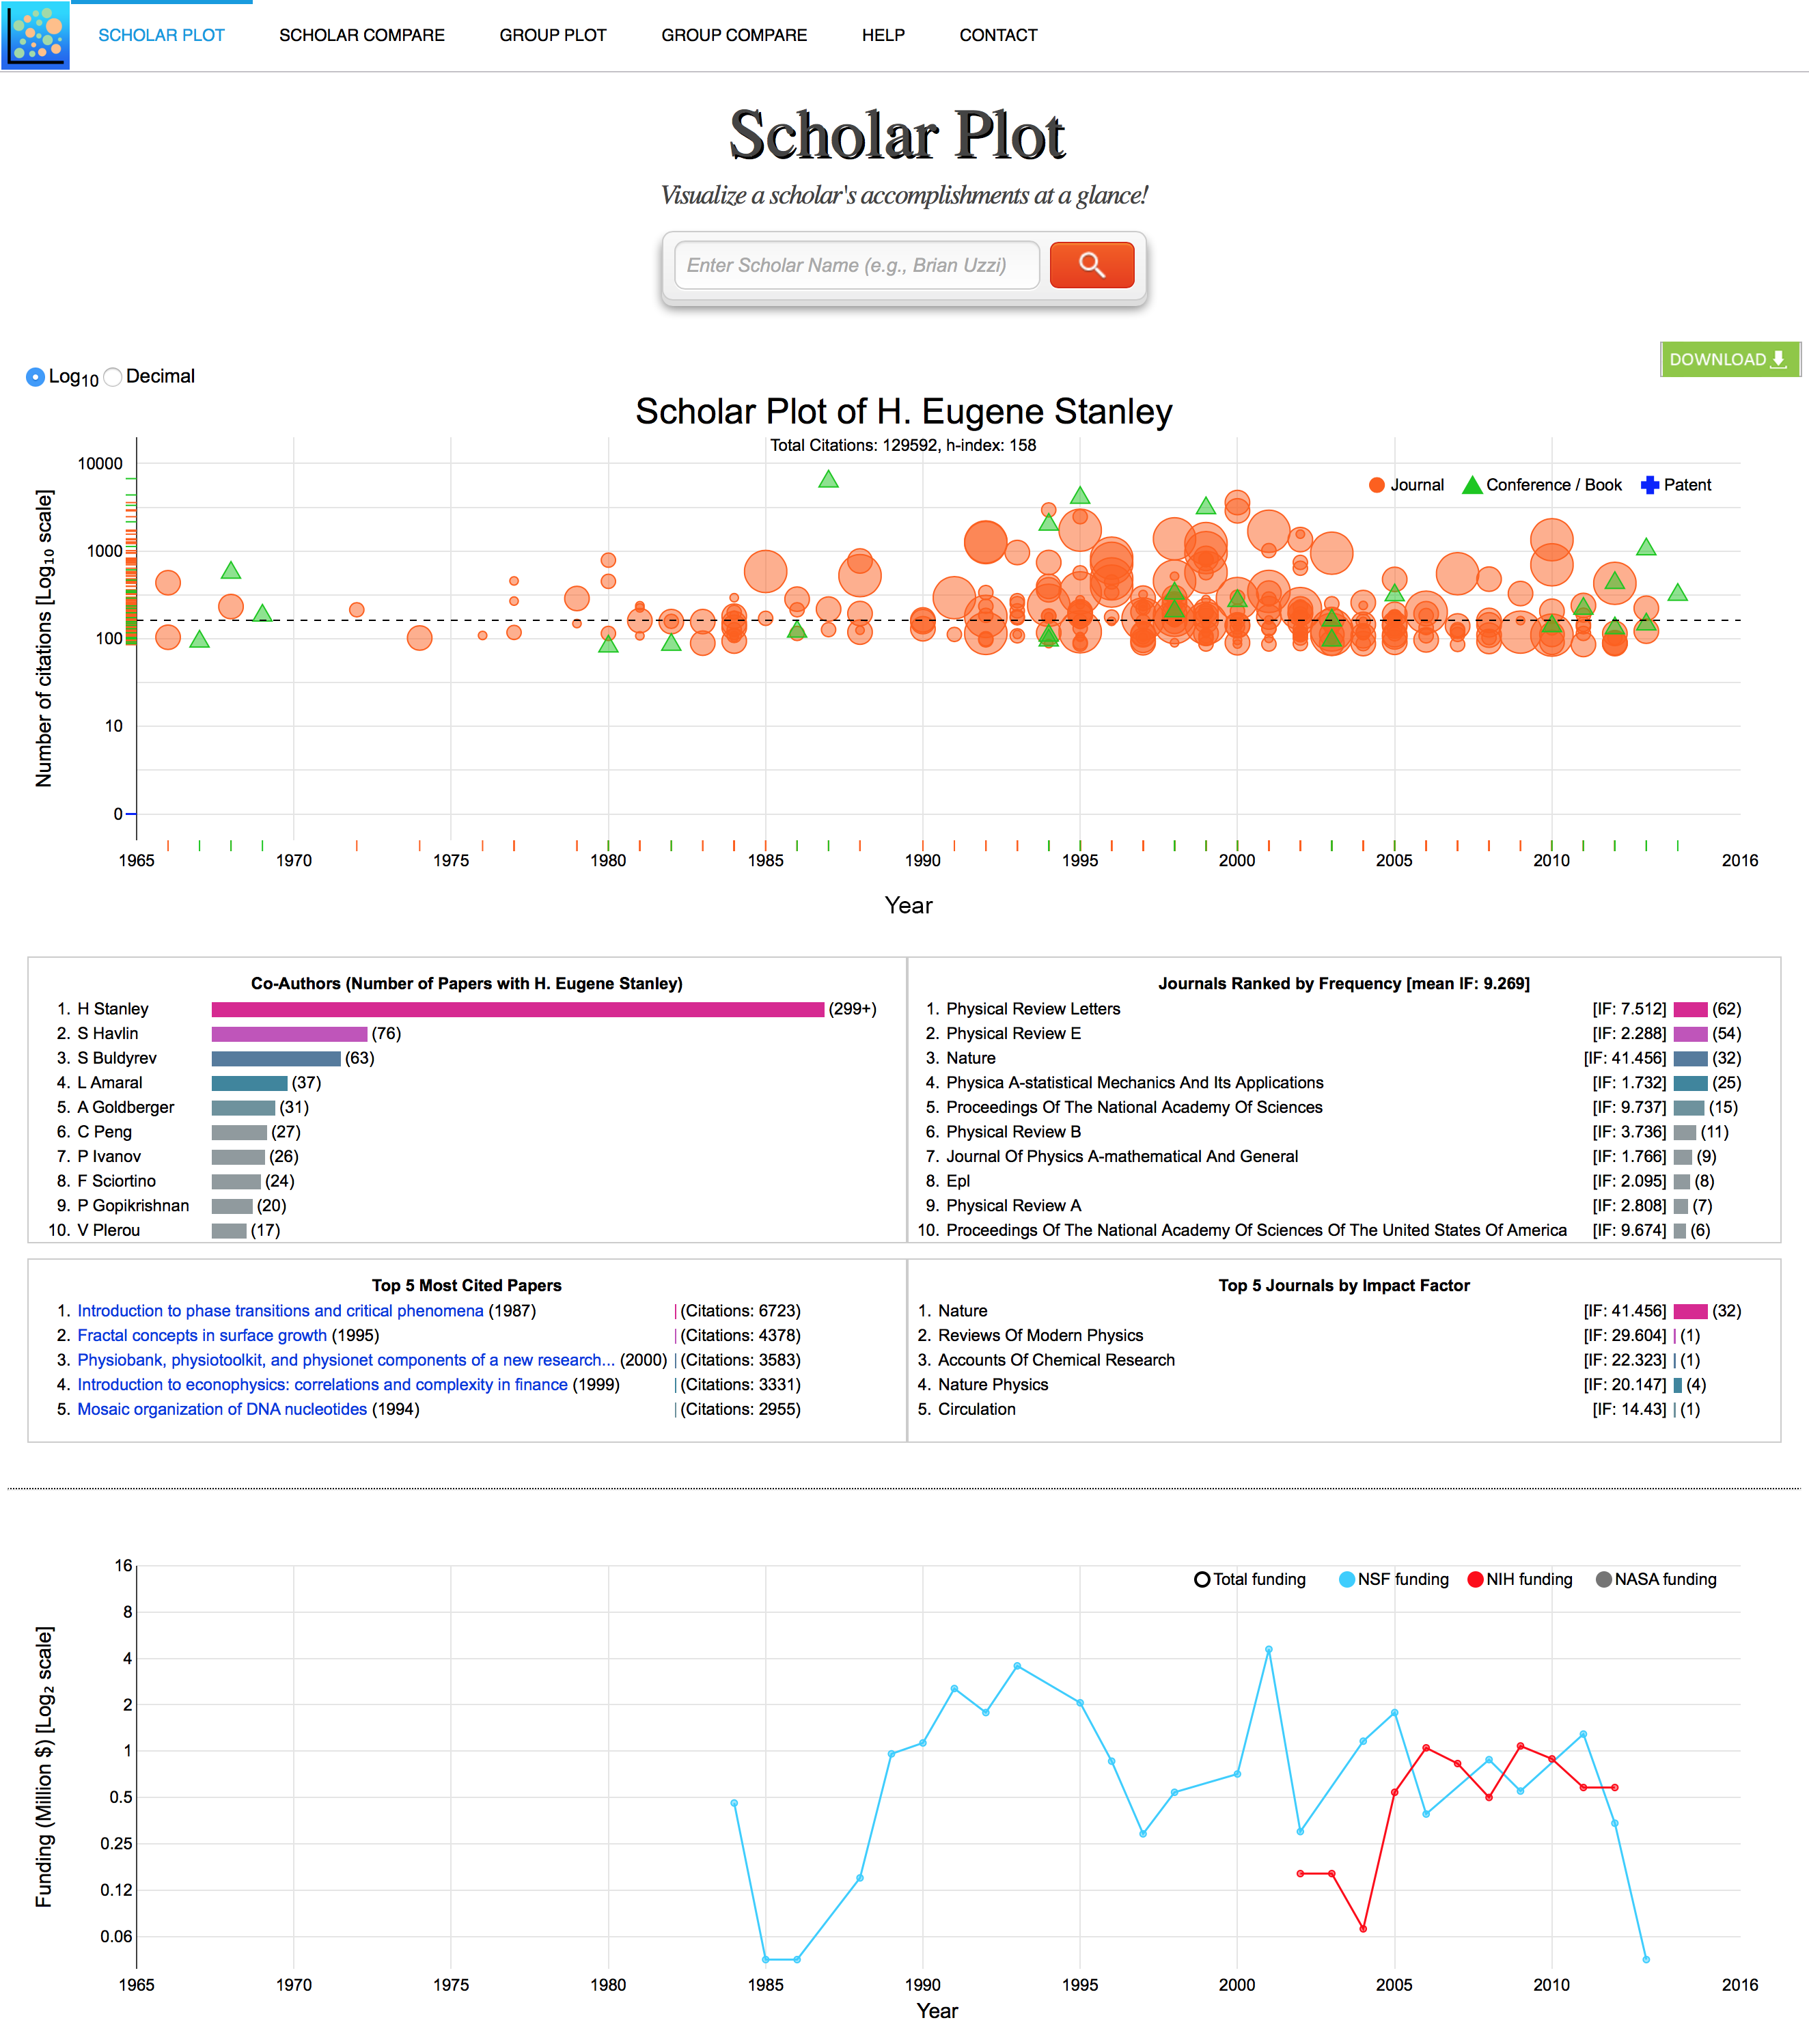
\includegraphics[width=1\textwidth]{figures/fig-Eugene-with-menu}
%     \caption{Base level Scholar Plot (SP) example - a famous physicist and interdisciplinary scientist with dozen of articles in \emph{Nature}. The summary panels in the middle were added after feedback from the focus group. Notice how this scholar's publication production exploded in sync with the commencement of substantial federal funding.}~\label{fig-publication} 
% \end{figure*} 

% ------------------------------------------------------------------
\subsection {Prestige of Product Venue: Pre-production Achievement}
% ------------------------------------------------------------------
Funded (and unfunded) research typically results in intellectual products. These are typically journal papers, conference proceedings papers, or books. Occasionally, intellectual products include patents or software packages, such as smartphone applications. Almost all intellectual products undergo review process, and the ones successfully passing this review process have inherent merit.  The review process criteria are not uniform. Moreover, publishing in different venues is associated with various degrees of difficulty. In journals, this difficulty is largely associated with the journal's impact factor (IF), as determined by Thomson Reuters - the higher the IF, the more difficult it is to be published in a journal, and the more valuable and prestigious a potential acceptance. For refereed conferences, the prestige is loosely associated with the venue's acceptance rate? the lower the acceptance rate, the more difficult it is to get into the conference proceedings, and the more prestigious the accomplishment. Unfortunately, there is no universally accepted ranking list for conferences, as is the case of the Thomson Reuters IF list for journals. Hence, it is not opportune to assign a numeric score to conference publications. The same applies for books, where evaluations are even more qualitative, and based on opinions about the perceived prestige of the publishing house. And, we are totally agnostic regarding pre-production credit, when it comes to patents and software products.
As a result, for the moment we use only IF to measure pre-production achievement. Based on the histogram analysis of the frequency of publications in the IF list of journals, we use four classes to group prestige. Different grouping may be adopted, however, depending on the analytics used. 

\begin{itemize}
\item CLASS-1: IF $<$ 2
\item CLASS-2: 2 $<=$ IF $<$ 4
\item CLASS-3: 4 $<=$ IF $<$ 16
\item CLASS-4: 16 $<$ IF
\end{itemize}



% \begin{figure*}
%     \centering
%     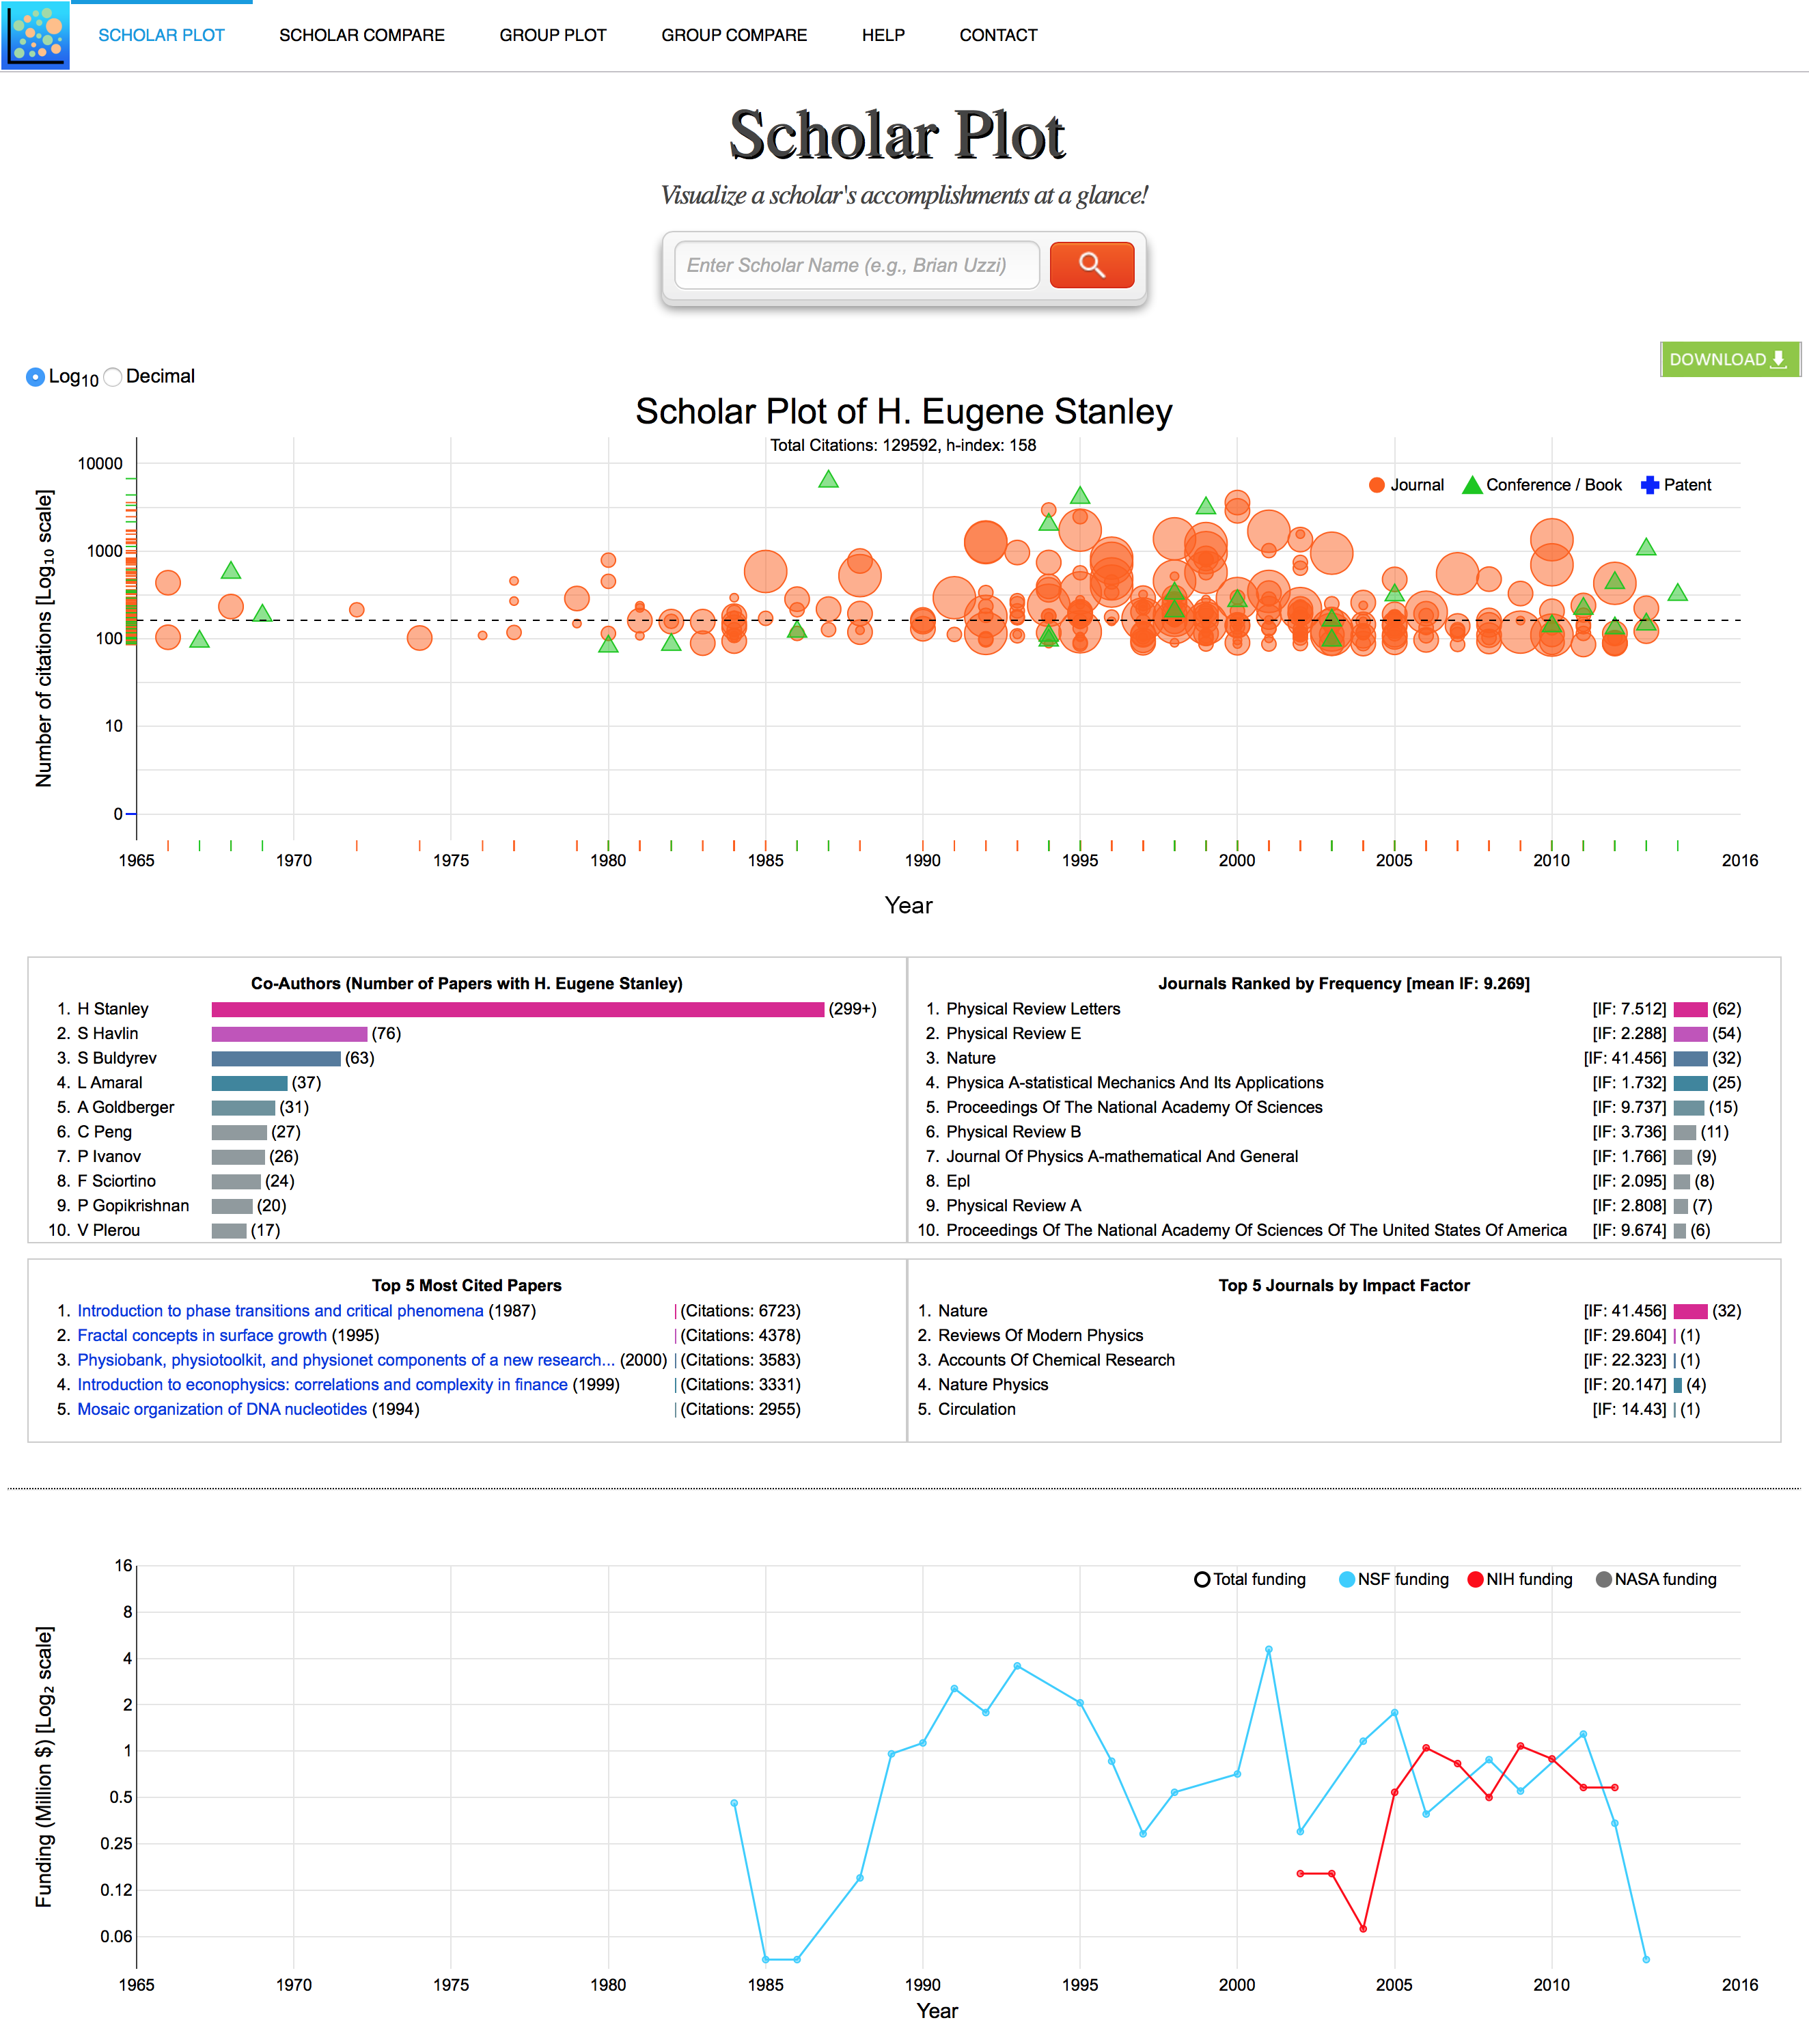
\includegraphics[width=1\textwidth]{figures/fig-Eugene-with-menu}
%     \caption{Base level Scholar Plot (SP) example - a famous physicist and interdisciplinary scientist with dozen of articles in \emph{Nature}. The summary panels in the middle were added after feedback from the focus group. Notice how this scholar's publication production exploded in sync with the commencement of substantial federal funding.}~\label{fig-publication} 
% \end{figure*} 

% ------------------------------------------------------------------
\subsection {Product Impact: Post-production Achievement}
% ------------------------------------------------------------------
Once a paper appears in a journal or conference proceedings, or a book appears in the market, it gets noticed and depending on how useful researchers find the concept or method contained therein, they may start using it, and citing its source in their own intellectual products. This practice constitutes impact, which is a sought-after outcome of the research process as the building block of scientific advances. There are several ways of measuring impact, but the most widely accepted is the citation count.

As different disciplines have different population sizes and publication practices, which may affect citation numbers, normalization is in order. This normalization can be any statistics. We prefer the quartile where the citation count of the academic entity's record belongs with respect to `all' the records in the specific discipline.  `All' here is commensurate to the selected reference, whether this is a university department or a set of departments across the United States. Needless to say that the original citation records need to be adjusted, taking into account the entity's age (if the entity is a physical person) or the number of individuals participating in the entity's personhood (if the entity is a group).


% ------------------------------------------------------------------
\subsection* {Putting it All Together}
% ------------------------------------------------------------------

The design is not only measurable, but also comprehensive, fair, and sensible. As an abstracted pattern, it holds true not only for academic production, but also for many other types of creative production. I considered representative cases to support the argument that this value system gives credit where credit is due, while at the same time it pinpoints the hidden truth that are not accounted for under the present heuristic and fuzzy evaluation processes. 

SINKHOLE: Take the case of a well-funded academic entity that churns out products appearing in low-level journals and collecting few citation hits. This entity deserves some credit for winning competitive grants. From the science policy point of view such an entity is a liability in the long run, as it acts like a sinkhole of public funds. The three-prong merit system captures the pros and cons of this case, highlighting their causal linking.

LEAN \& MEAN: In contradistinction, consider an entity that has moderate funding but publishes articles in highly prestigious journals that receive many citation hits. From the science policy point of view, this is a `lean and mean' academic machine, as with moderate resources achieves maximum results. Every relevant funding agency would like to give to this entity more funding, as it represents a great investment. The three-prong merit system captures the pros of this case, highlighting their causal linking.

ODDBALL: Consider an entity that publishes highly novel concepts in big journals. The concepts attract attention for their creative power but find no use for the moment, receiving few citation hits. The fact that the concepts did not find an immediate application does not detract from their intellectual worth, which is captured by the pre-production merit criterion. The three-prong merit system captures the pros and cons of this case, highlighting their causal linking.

UNASSUMING HERO: Consider an entity that publishes specialized methods in solid transaction level journals. These methods find wide applicability in the relevant disciplinary communities and are widely cited. This entity did not receive any huge pre-production merit. However, its post-production impact more made up for it. The three-prong merit system captures the pros and cons of this case, highlighting their causal linking.


% ------------------------------------------------------------------
\subsection {Academic Garden Flower Diagram}
% ------------------------------------------------------------------

The flower was chosen as the visual metaphor for the performance of an academic entity. A nice looking flower is highly desirable, and so is a meritorious academic entity. Structurally, the stem, and disc make up a flower. We defined: (a) the width of the stem to be commensurate to the academic entity's funding; (b) the height of the stem to be commensurate to the academic entity's citation record; and (c) the diameter of its disc to be commensurate to the prestige of the venues where it publishes. 
\begin{figure}[H]
    \centering
    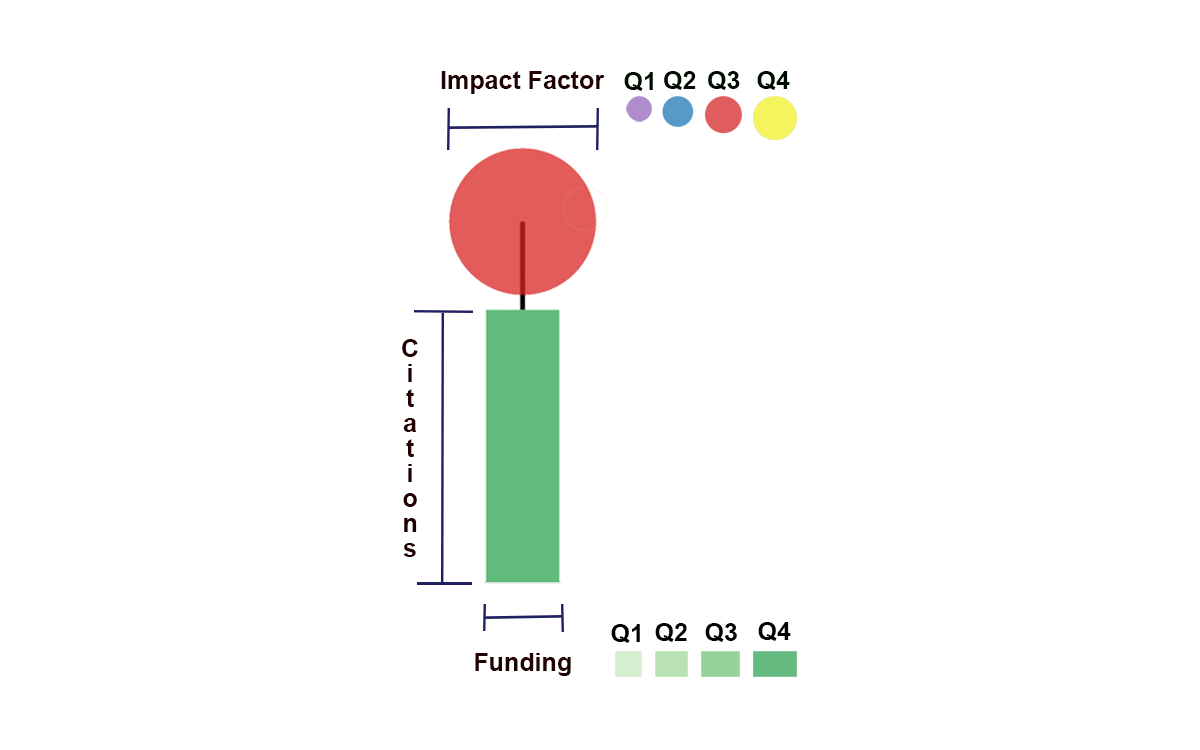
\includegraphics[width=1\textwidth]{figures/fig-flower.png}
    \caption{A wider stem means that a flower has the necessary support to grow. The width of each stem in the plot indicates the level of funding the scholar has received. A higher quartile of funding is represented by a wider stem and a darker green color. As a flower grows its stem heightens. The length of each stem in the plot represents a scholar's total number of citations.}~\label{fig-flower-diagram}
\end{figure}


\begin{figure}[!htb]
    \centering
    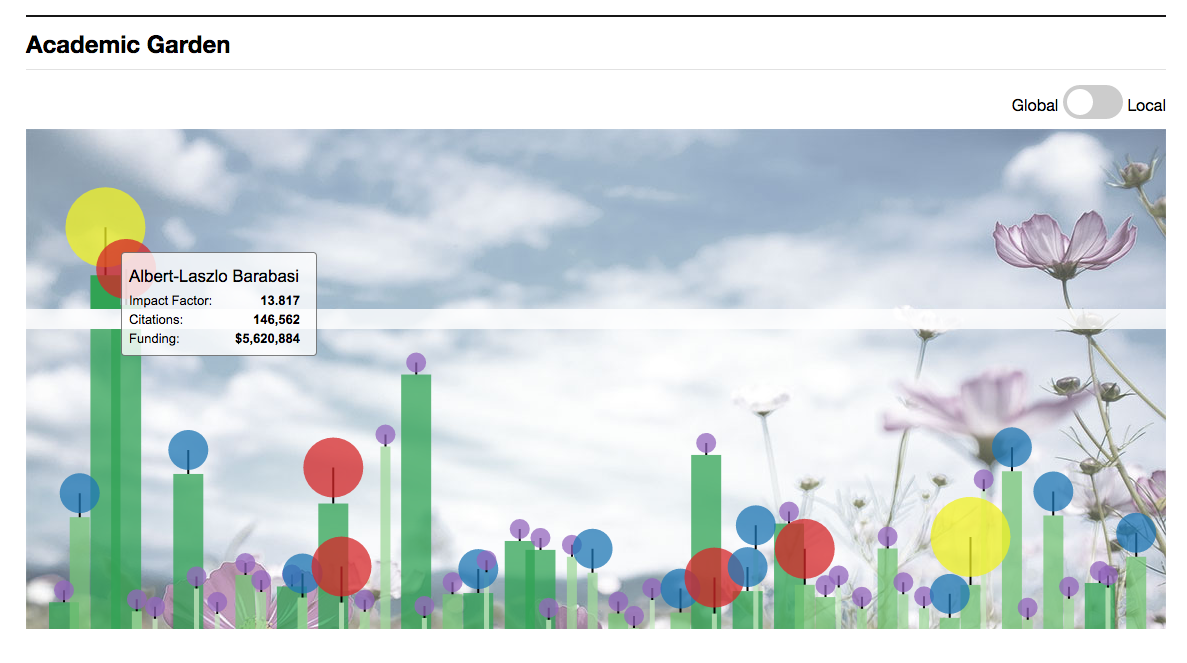
\includegraphics[width=1\textwidth]{figures/fig-AG-global.png}
    \caption{Academic Garden example of Global Scale - Computer and Information Science at Northeastern University.}~\label{fig-AG-global}
\end{figure}

\begin{figure}[!htb]
    \centering
    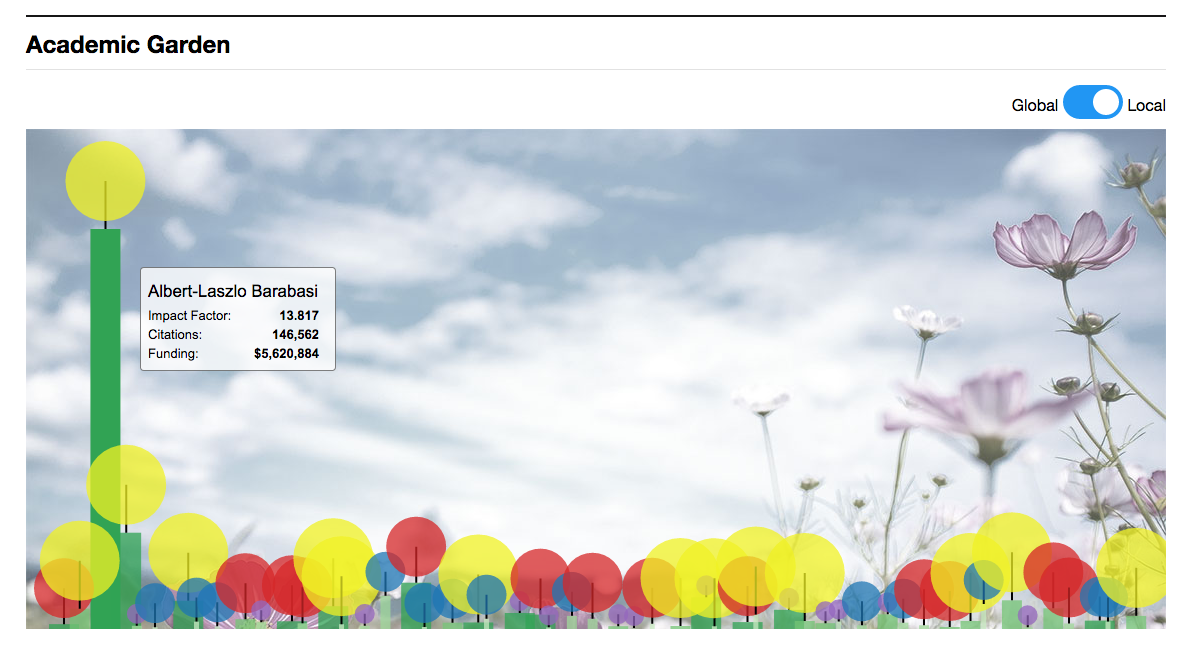
\includegraphics[width=1\textwidth]{figures/fig-AG-local.png}
    \caption{Academic Garden example of Local Scale - Computer and Information Science at Northeastern University.}~\label{fig-AG-global}
\end{figure}




















